\chapterimage{05_Uklon.jpg} % Chapter heading image

\chapter{Uklon}
\label{chap:Uklon}
V tem poglavju bomo spoznali enega najznačilnejših pojavov valovne 
optike -- uklon. Zapisali bomo splošni uklonski integral in obravnavali
dva približka, Fraunhoferjevega in Fresnelovega. Z izračunom 
bomo pojasnili značilne uklonske slike in zapisali uklonsko
omejeno ločljivost optičnih naprav. Na koncu poglavja sledi matematično
zahtevnejša izpeljava Kirchhoffovega uklonskega integrala. 

\section{Uklonski integral}
\label{chap:uklint}
Svetloba se uklanja, kadar vpada na oviro, katere velikost je primerljiva z valovno  
dolžino svetlobe, ali se širi skozi podobno veliko odprtino v zaslonu. 
V geometrijski optiki se svetloba širi po ravnih črtah, ki po 
najkrajši poti povezujejo začetno in končno točko. V tej sliki za oviro 
nastane ostra senca, v katero se svetloba ne širi. Po uklonski teoriji
svetloba seže deloma tudi v območje sence. Poleg tega, da se valovanje širi
v območje geometrijske sence za ovirami, se v njem pojavijo ojačitve
in oslabitve, ki predstavljajo značilne uklonske slike.

Naj ravno sinusno potujoče valovanje vpada na zaslon, v katerem je majhna odprtina.
Ta zaslon imenujemo objektni zaslon. Iščemo uklonsko sliko, ki nastane
za odprtino na tako imenovanem opazovalnem zaslonu (glej sliko~\ref{fig:05_shema}).
Pri tem  zanemarimo vektorsko naravo polja oziroma
polarizacijo in jakost električnega polja obravnavamo kot skalarno količino.

\begin{figure}[ht]
\centering
\def\svgwidth{90truemm} 
\input{slike/05_skica01.pdf_tex}
\caption{Ravni valovi vpadajo na objektni zaslon, v katerem je odprtina. 
Na opazovalnem zaslonu v točki $P_0$ opazujemo jakost električnega polja v
odvisnosti od vpadnega polja v točki $P$.}
\label{fig:05_shema}
\end{figure}

Naša naloga je poiskati jakost električnega polja v točki $P_0$ na opazovalnem zaslonu, 
do katere vodi vektor $\mathbf{r}_0$, v odvisnosti od vrednosti polja v točki $P$
na objektnem zaslonu, do katerega vodi vektor $\mathbf{r}$.

Po Huygensovem načelu iz vsake točke $P$ v odprtini izhaja sekundarno krogelno valovanje, 
katerega amplitudo določa polje, ki vpada na objektni zaslon. Če je vpadno valovanje
ravni val, velja $E(\mathbf{r}) = E_0$ za vsak $\mathbf{r}$. Za nastanek slike
v točki $P_0$  na opazovalnem zaslonu seštejemo prispevke sekundarnih
polj iz vseh točk odprtine v objektnem zaslonu. 

Uklonsko sliko v točki $P_0$ tako z enačbo zapišemo kot:
\boxeq{eq:05_01}{
E_{P0} = E (\mathbf{r}_0) = \int_{S_A} \frac{1}{i\lambda} 
E_0~\frac{e^{ikR(\mathbf{r})}}{R(\mathbf{r})}~ dS,
}
pri čemer integriramo po celotni površini odprtine $S_A$. Ulomek v integralu predstavlja
krajevni del krogelnih valov, $\lambda$ pa je valovna dolžina vpadne svetlobe. Predfaktor
v obliki $1/i\lambda$ bomo izpeljali v razdelku~\ref{chap:Kirchhoff}.
\begin{remark}
Uklonski integral je prvotno zapisal Fresnel, vendar je namesto predfaktorja 
$1/i\lambda$ uvedel eksperimentalno določeno konstanto. Predfaktor $1/i\lambda$ je 
izpeljal Kirchhoff. Popolnejši zapis predfaktorja je oblike $ \chi(\mathbf{r})/i\lambda$,
pri čemer $\chi$ predstavlja smerni faktor. Kadar je značilna razsežnost odprtine v 
objektnem zaslonu $d$ bistveno manjša od oddaljenosti do opazovalnega zaslona, 
je $\chi \approx 1$ in predfaktor se prevede na zapisano obliko. 
\end{remark}

Namesto integracije sekundarnega valovanja po območju odprtine $A$, lahko vpeljemo
tako imenovano aperturno funkcijo $f(\mathbf{r})$. Njena vrednost je na mestu odprtine enaka $1$,
sicer je enaka $0$. Zapis z aperturno funkcijo omogoči integracijo po celotni dvodimenzionalni
ploskvi, ki opisuje objektni zaslon. Zapis je uporaben tudi za splošen primer, ko je zaslon
delno prozoren in le delno prepušča svetlobo. Polje v ravnini objektnega zaslona potem zapišemo kot:
\beq
E(\mathbf{r}) = f(\mathbf{r})E_0.
\label{eq:05_02}
\eeq
Določimo koordinatni sistem na objektni in opazovalni ravnini, ki ju bomo potrebovali
za izračun uklonskega integrala. Objektno ravnino
opišemo kot ravnino s koordinatama $x$ in $y$, vzporedno opazovalno ravnino pa kot ravnino
s koordinatama $\xi$ in $\eta$. Izhodišči obeh koordinatnih sistemov naj ležita 
na skupni osi $z$, ki jo imenujemo optična os sistema (glej sliko~\ref{fig:05_koordinate})
in je pravokotna na obe ravnini.
\begin{figure}[ht]
\centering
\def\svgwidth{120truemm} 
\input{slike/05_koordinate.pdf_tex}
\caption{Optična os sistema (os $z$) povezuje središči obeh ravnin, objektne ($x,y$) in 
opazovalne ($\xi, \eta$). Razdalja med točko v odprtini $P$ in točko na opazovalnem zaslonu $P_0$
je $R$.}
\label{fig:05_koordinate}
\end{figure}

Točko $P$ na objektnem zaslonu opišemo s krajevnim vektorjem:
\beq
P: \mathbf{r} = (x,y,0),
\label{eq:05_03}
\eeq
točko $P_0$ na opazovalnem zaslonu pa s krajevnim vektorjem:
\beq
P_0: \mathbf{r}_0 = (\xi,\eta,z_0).
\label{eq:05_04}
\eeq
Uporabimo uklonski integral (enačba~\ref{eq:05_01}) in zapišemo:
\boxeq{eq:05_05}{
E(\xi, \eta, z_0) = \frac{1}{i\lambda} \int_{-\infty}^{\infty}
\int_{-\infty}^{\infty} f(x,y) E_0~\frac{e^{ikR}}{R}~ dx\,dy.
}
V izrazu za krogelne valove nastopa razdalja $R$ med točkama $P$ in $P_0$, za
katero velja:
\beq
R = \sqrt{(\xi-x)^2 + (\eta - y)^2 + z_0^2}.
\label{eq:05_06}
\eeq

Natančna obravnava uklonskega integrala je zelo zahtevna, zato se poslužujemo približkov.
Glede na to, kako natančno obravnavamo izraz za $R = R(x,y,\xi, \eta, z_0)$ v uklonskem
integralu (enačba~\ref{eq:05_05}), ločimo med različnimi uklonskimi približki. Najbolj 
znana sta Fraunhoferjev in Fresnelov približek.

\section{Fraunhoferjev uklon}
O Fraunhoferjevem uklonu oziroma natančneje Fraunhoferjevem uklonskem približku govorimo,
kadar razdaljo $R$ med točko v odprtini in točko na zaslonu v uklonskem integralu 
(enačba~\ref{eq:05_05}) razvijemo do prvega reda. Zapišemo:
\beq
R = \sqrt{(\xi-x)^2 + (\eta - y)^2 + z_0^2} =
\sqrt{\xi^2+\eta^2 +z_0^2 - 2\xi x - 2 \eta y + x^2 + y^2}.
\label{eq:05_07}
\eeq
Vpeljemo $R_0$ kot razdaljo od izhodišča do točke na zaslonu, za katero velja 
$R_0^2 = \xi^2 + \eta^2 + z_0^2$ (glej sliko~\ref{fig:05_koordinate}). Nato korensko
funkcijo razvijemo do prvega reda in ohranimo le člene, ki so linearni v $x$ in $y$. 
Dobimo:
\beq
R = \sqrt{R_0^2 \left(1 - \frac{2\xi x}{R_0^2} - \frac{2\eta y}{R_0^2} + \frac{x^2+y^2}{R_0^2}
\right)} \approx 
R_0 - \frac{\xi x}{R_0} - \frac{\eta y}{R_0}.
\label{eq:05_10}
\eeq
Člen v uklonskem integralu, ki opisuje krogelne monokromatske valove, z upoštevanjem razvoja
(enačba~\ref{eq:05_10}) zapišemo kot:
\beq
\frac{e^{ikR}}{R} \approx \frac{e^{ikR_0} e^{-ik\xi x /R_0} e^{-ik\eta y/R_0}}{R_0}.
\label{eq:05_11}
\eeq
Ker je odvisnost od koordinat $x$, $y$, $\xi$ in $\eta$ v imenovalcu znatno 
šibkejša kot v števcu, smo jo v imenovalcu zanemarili. 

Enačba~(\ref{eq:05_05}) se z upoštevanjem razvoja prepiše v:
\boxeq{eq:Fraunhofer}{
E(\xi, \eta, z_0) = \frac{1}{i\lambda} 
\frac{E_0 e^{ikR_0}}{R_0}
\int_{-\infty}^{\infty} \int_{-\infty}^{\infty} 
f(x,y)~ e^{-ik\xi x /R_0} e^{-ik\eta y/R_0} dx\,dy.
}

Vpeljemo še smerna oziroma uklonska kota, za katera privzamemo, da sta majhna:
\beq
\sin \vartheta_\xi \approx \vartheta_\xi = \frac{\xi}{R_0}
\qquad \mathrm{in}
\qquad
\sin \vartheta_\eta \approx \vartheta_\eta = \frac{\eta}{R_0},
\label{eq:05_13}
\eeq
ter z njimi povezani prostorski frekvenci:
\beq
\omega_\xi = k \vartheta_\xi
\qquad \mathrm{in}
\qquad
\omega_\eta = k \vartheta_\eta.
\label{eq:05_14}
\eeq
Pogosto naredimo še približek $R_0 \approx z_0$, s katerim uklonski integral 
v Fraunhoferjevem približku zapišemo kot:
\boxeq{eq:Fraunhoferjev}{
E(\omega_\xi,\omega_\eta) = \frac{1}{i\lambda} \frac{E_0 e^{ikz_0}}{z_0}
\int_{-\infty}^{\infty}
\int_{-\infty}^{\infty} f(x,y) e^{-i\omega_\xi x} e^{-i \omega_\eta y} dx\, dy.
}

Iz enačbe~(\ref{eq:Fraunhoferjev}) je razvidno, 
da je uklonska slika objekta v Fraunhoferjevem uklonskem približku
enaka 2D Fourierevi transformiranki aperturne funkcije tega objekta. 

\begin{remark}
Uklonski integral smo zapisali za splošno aperturno funkcijo $f(x,y)$. Ta lahko
opisuje odprtino v zaslonu ali pa oviro, na katero svetloba vpada. 
Babinetovo načelo (po francoskem fiziku Jacquesu Babinetu, 1794--1872) pravi, 
da je uklonska slika ovire enaka uklonski sliki odprtine v zaslonu, 
ki je enake oblike in enake velikosti kot ovira. 
\end{remark}

\subsection*{Fresnelovo število}
Poiščimo kriterij, ki določa, kdaj lahko uporabimo navedeni približek. Spomnimo se, da smo
v razvoju izraza za $R$ zanemarili kvadratni člen (enačba~\ref{eq:05_10}), ki 
nastopa v obliki $\exp(ik(x^2 + y^2)/2R_0)$ in torej prinaša nek dodatni fazni zamik. 
Da je ta člen res zanemarljiv, mora za vse vrednosti $x$ in $y$ znotraj odprtine veljati:
\beq
\frac{k(x^2+y^2)}{2R_0} \ll 2 \pi.
\label{eq:05_15}
\eeq
Privzamemo, da je $(x^2+y^2)_\mathrm{max} = d^2$, pri čemer $d$ meri karakteristično razsežnost 
odprtine v objektnem zaslonu. Sledi:
\beq
\frac{kd^2}{2R_0}  = \frac{2\pi}{\lambda}\frac{d^2}{2R_0}\ll 2 \pi.
\label{eq:05_16}
\eeq
Vpeljemo Fresnelovo število $F$ kot:
\beq
F  = \frac{d^2}{\lambda R_0}.
\label{eq:05_17}
\eeq
Fraunhoferjev uklonski približek je veljaven, kadar velja:
\beq
F \ll 1. 
\label{eq:05_18}
\eeq
Pogoj je ekvivalenten zahtevi, da je: 
\beq
R_0 \gg \frac{d^2}{\lambda}.
\label{eq:05_19}
\eeq
Tipične vrednosti $R_0 \approx z_0$  morajo biti za veljavnost Fraunhoferjevega 
približka dosti večje od dimenzij odprtine, zato 
Fraunhoferjevemu približku rečemo tudi približek daljnjega polja. 

\begin{example}{\bf Veljavnost Fraunhoferjevega približka.}
\label{ex:fh}
Naj bo valovna dolžina vpadne svetlobe $\lambda=500~\si{nm}$. Če je tipična 
razsežnost odprtine $d = 1~\si{\micro\metre}$, je veljavnost 
Fraunhoferjevega približka pri oddaljenosti od zaslona 
$R\gg 2~\si{\micro\metre}$. Pri razsežnosti
$d = 10~\si{\micro\metre}$ velja $R\gg 200~\si{\micro\metre}$, 
pri $d = 100~\si{\micro\metre}$ velja $R\gg 2~\si{\centi\metre}$ in 
pri $d = 1~\si{\milli\metre}$ velja Fraunhoferjev približek za
$R\gg 2~\si{\metre}$. Pri majhnih odprtinah je torej Fraunhoferjev približek
preprosto izpolniti, že pri milimetrskih odprtinah
pa mora biti zaslon oddaljen vsaj nekaj metrov. 
\end{example}

Preden obravnavamo primere Fraunhoferjevega uklona, si oglejmo še interpretacijo 
Fraunhoferjevega približka. Zamislimo si enodimenzionalno režo, ki se razteza v smeri 
osi $x$. Fazni zamik sekundarnih sferičnih valov, ki izvirajo iz reže pri danem $x$ 
in se zberejo v eni točki na zaslonu, se po enačbi~(\ref{eq:05_11}) spreminja z lego $x$ kot:
\beq
\Delta \phi = \frac{k \xi x}{R_0}.
\label{eq:05_20}
\eeq
Primerjamo to z faznim zamikov ravnih valov, ki potujejo v smeri $\vartheta_\xi \approx
\xi/R_0$ glede na os $z$:
\beq
\Delta \phi = k x \vartheta_\xi.
\label{eq:05_21}
\eeq
Vidimo, da sta fazna zamika (enačbi~\ref{eq:05_20} in \ref{eq:05_21}) enaka. 
V Fraunhoferjevem približku je torej uklonjeno valovanje
enako ravnim valovom, ki se širijo pod kotom $\vartheta_\xi$ 
(skica~\ref{fig:05_ravnivalovi}).
\begin{figure}[h]
\centering
\def\svgwidth{75truemm} 
\input{slike/05_ravnivalovi.pdf_tex}
\caption{V Fraunhoferjevem približku so uklonjeni valovi ravni valovi. Približek
velja za velike oddaljenosti od zaslona, zato mu pravimo tudi približek
daljnjega polja.}
\label{fig:05_ravnivalovi}
\end{figure}

Za veljavnost Fraunhoferjevega približka mora biti opazovalni zaslon zelo
oddaljen od odprtine, na kateri se svetloba uklanja. Tej nepraktični 
postavitvi se lahko izognemo, če za objektni zaslon postavimo zbiralno 
lečo in uklonsko sliko opazujemo v njeni goriščni ravnini (slika~\ref{fig:05_2DFourier}). 
Zbiralna leča namreč snop vzporednih žarkov zbere v eni 
točki v goriščni ravnini leče. Na podoben način na vpadni strani svetlobo, ki 
izhaja iz točkastega svetila v gorišču leče, preslikamo v snop vzporednih žarkov (kolimiramo)
in dosežemo enakomerno osvetlitev
objektnega zaslona z vpadnim snopom ravnih valov.
Z dodatim ustreznim spektralnim filtrom ustvarimo 
monokromatsko valovanje.
\begin{figure}[ht]
\centering
\def\svgwidth{80truemm} 
\input{slike/05_2DFourier.pdf_tex}
\caption{Ravne valove, ki nastanejo pri Fraunhoferjevi uklonski sliki, lahko opazujemo v
veliki oddaljenosti, ali pa jih zberemo z lečo v goriščni ravnini. Tako v goriščni
ravnini nastane 2D-Fouriereva transformiranka aperturne funkcije.}
\label{fig:05_2DFourier}
\vglue-5truemm
\end{figure}

\begin{remark}
Opisani sistem je analogna naprava za izračun 2D-Fouriereve transformacije izbranega 
delno prozornega objekta ali vzorca.
\end{remark}

\begin{example}{\bf Fraunhoferjev uklon na reži širine $d$.}
Obravnavajmo uklon svetlobe z valovno dolžino $\lambda$, ki v obliki ravnih valov 
vpada na zaslon z režo širine $d$. Uklonsko sliko na oddaljenem opazovalnem zaslonu
izračunamo iz enačbe~(\ref{eq:Fraunhoferjev}), pri čemer je funkcija $f(x)$ enaka 1 za
$-d/2<x<d/2$, sicer je 0. Integral po smeri $y$ in ostale predfaktorje združimo
v konstanto $K$ in zapišemo:
\beq
E(\omega_\xi) = K \int_{-d/2}^{d/2} e^{-i\omega_\xi x} dx \approx
\frac{K}{-i\omega_\xi}\left(e^{-i\omega_\xi d/2}- e^{i\omega_\xi d/2}\right)\!\!.
\label{eq:05_22}
\eeq
Z upoštevanjem izraza za $\sin(x)$ dobimo:
\beq
E(\omega_\xi) = \frac{2K}{\omega_\xi} \sin\left(\omega_\xi d/2\right) = 
Kd\,
\frac{\sin\left(\omega_\xi d/2\right)}{\omega_\xi d/2}.
\label{eq:05_23}
\eeq
Gostota svetlobnega toka uklonjene svetlobe na opazovalnem zaslonu je tako:
\boxeq{eq:uklon1reza}{
j(\vartheta) = j_0 \left(\frac{\sin\left(kd\sin \vartheta/2\right)}{kd\sin\vartheta/2}\right)^2\!\!,
}
pri čemer so $k$ valovno število, $d$ širina reže in $\vartheta$ uklonski kot. Gostoto
toka smo normirali, tako da je v smeri naravnost (pri $\vartheta = 0$) enaka $j_0$.
Relativna intenziteta uklonjene svetlobe v odvisnosti od uklonskega kota $\vartheta$ 
je prikazana na sliki~\ref{fig:05_1Reza}.
\begin{figure}[ht]
\centering
\def\svgwidth{90truemm} 
\input{slike/05_Fraunhofer_1.pdf_tex}
\caption{Zgoraj: simulacija uklonske slike laserskega snopa na eni uklonski reži. Spodaj:
Odvisnost relativne intenzitete uklonjene svetlobe v odvisnosti od uklonskega kota.}
\label{fig:05_1Reza}
\end{figure}
\begin{figure}[ht]
\centering
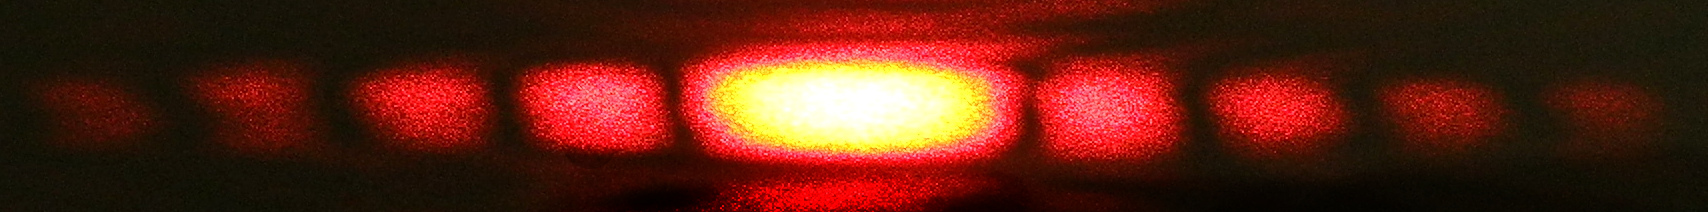
\includegraphics[width=90truemm]{slike/05_photos_Fraunhofer.jpg}
\caption{Fotografija Fraunhoferjeve uklonske slike na eni reži}
\label{fig:05_FranuhoferFoto}
\end{figure}

V smeri naprej je intenziteta uklonjene svetlobe največja, nato z naraščajočim
kotom pojema, dokler ne doseže vrednosti 0. Pri večjih kotih se pojavijo stranski
vrhovi, vendar je njihova intenziteta znatno manjša kot v osrednjem vrhu. 

Uklonske kote, pri 
katerih se pojavijo oslabitve, izračunamo preprosto iz enačbe~(\ref{eq:uklon1reza}), tako da
števec postavimo na nič. Sledi:
\beq
kd \sin \vartheta/2 = N\pi \qquad \mathrm{in} \qquad \sin \vartheta = \frac{N\lambda}{d},
\label{eq:05_24}
\eeq
pri čemer je $N$ celo število. Lego vrhov je treba določiti numerično, saj 
vrhovi ne ležijo točno na sredini med dvema oslabitvama. Povejmo še, da 
se z naraščajočo širino reže $d$ uklonski vrhovi gostijo in uklonska slika oža
(slika~\ref{fig:05_Rezad}\,a). Po drugi strani se pri zelo ozkih režah uklonski 
vrhovi razširijo in celotna uklonska slika seže globoko v območje sence 
(slika~\ref{fig:05_Rezad}\,b).
\begin{figure}[ht]
\centering
\def\svgwidth{110truemm} 
\input{slike/05_Fraunhofer_d.pdf_tex}
\caption{Shema Fraunhoferjeve uklonske slike na eni reži. 
Širša reža da razmeroma ozke vrhove in ozko
uklonsko sliko (a), ozka reža pa široke uklonske vrhove, ki sežejo globoko v območje 
geometrijske sence (b).}
\label{fig:05_Rezad}
\end{figure}
\vglue-5truemm

\end{example}

\begin{example}{\bf Fraunhoferjev uklon na pravokotni reži.}
 V prejšnjem primeru smo obravnavali enodimenzionalni primer uklona, v tem
 primeru pa integral razširimo v dve dimenziji. Ker sta integrala v izrazu
 za uklonsko sliko (enačba~\ref{eq:Fraunhoferjev}) povsem ekvivalentna, 
 lahko rezultat preprosto zapišemo. Za pravokotno režo z merama 
 $a$ v smeri $x$ in $b$ v smeri $y$ uklonsko sliko zapišemo kot:
 \beq
 j = j_0 \left(\frac{\sin\left(ka\sin \vartheta_\xi/2\right)}{ka\sin\vartheta_\xi/2}\right)^2
 \left(\frac{\sin\left(kb\sin \vartheta_\eta/2\right)}{kb\sin\vartheta_\eta/2}\right)^2\!\!,
 \eeq
 pri čemer smo izhodišče postavili na sredino odprtine. Uklonski vzorec
 je prikazan na sliki~\ref{fig:05_pravokot}.
 \begin{figure}[ht]
\centering

\includegraphics[width=100truemm]{slike/05_pravokot.png}
\caption{Simulacija uklonske slike na pravokotni reži
za razmerje stranic $a:b = 1:2$.}
\label{fig:05_pravokot}
\end{figure}
\vglue-5truemm

\end{example}

\begin{example}{\bf Fraunhoferjev uklon na sistemu $N$ vzporednih rež.}
Naj bo v objektni ravnini $N$ vzporednih rež debeline $d$, perioda ponavljanja
rež pa naj bo $D$. Izračunajmo uklonsko sliko, ki nastane na opazovalnem zaslonu.

Podobno kot smo izračunali uklonsko sliko na eni reži, izračunamo tudi uklonsko sliko
na več vzporedih režah. Prepustnostna funkcija $f$ je enaka 1 v vsaki reži, med
režami in zunaj območja rež pa je enaka 0. Zapišemo:
\beq
E(\omega_\xi) = K
\left( \int_{-d/2}^{d/2} e^{-i\omega_\xi x} dx + \int_{D-d/2}^{D+d/2} e^{-i\omega_\xi x} dx +
\int_{2D-d/2}^{2D+d/2} e^{-i\omega_\xi x} dx + ... \right)\!\!.
\label{eq:05_25}
\eeq
Integrale izračunamo in dobimo:
\beq
E(\omega_\xi) = \frac{K}{-i\omega_\xi}
\left(e^{-i\omega_\xi d/2}- e^{i\omega_\xi d/2} \right) \left(1 + e^{-i\omega_\xi D} + 
e^{-i\omega_\xi 2 D} + ...\right)\!.
\label{eq:05_26}
\eeq
Geometrijsko vrsto v oklepaju seštejemo, uporabimo izraz za sinus in dobimo:
\beq
E(\omega_\xi) = Kd
\frac{e^{-iN\omega_\xi D/2}} {e^{-i\omega_\xi D/2}}
\frac{\sin(\omega_\xi d/2)}{\omega_\xi d/2} 
\frac{\sin(N\omega_\xi D/2)}{\sin(\omega_\xi D/2)}.
\label{eq:05_27}
\eeq
Gostota svetlobnega toka uklonjene svetlobe na opazovalnem zaslonu je tako:
\boxeq{eq:uklonNrez}{
j(\vartheta) = j_0 \left(\frac{\sin\left(kd\sin\vartheta/2\right)}{kd\sin\vartheta/2}\right)^2
\left(\frac{\sin\left(NkD\sin\vartheta/2\right)}{\sin\left(kD\sin\vartheta/2\right)}\right)^2\!\!.
}
Prvi oklepaj imenujemo strukturni faktor $S(\vartheta)$ in določa ovojnico 
uklonske slike. Enak je uklonski sliki za eno samo režo debeline $d$ 
(enačba~\ref{eq:uklon1reza}). 
Drugi oklepaj imenujemo mrežni faktor $M(\vartheta)$ in je odvisen od števila
in razporeditve rež (glej sliko~\ref{fig:05_Nrez}). 

\begin{figure}[ht]
\centering
\def\svgwidth{140truemm} 
\input{slike/05_Fraunhofer_N.pdf_tex}
\caption{Fraunhoferjeva uklonska slika na $N$ vzporednih režah. 
Primer je narisan za $N=5$ rež in $D=3d$. Strukturni faktor $S$ (modra) je 
enak kot uklonska slika ene reže. Produkt med strukturnim faktorjem in mrežnim
faktorjem $M$ (zelena) da celotno uklonsko sliko (rdeča). Nad izračunano
uklonsko sliko je simulacija uklonske slike laserskega snopa na enaki uklonski oviri.
Parameter $x = d\sin \vartheta/\lambda$.}
\label{fig:05_Nrez}
\end{figure}

Glavne vrhove v uklonski sliki dobimo, kadar je imenovalec mrežnega faktorja enak nič in velja:
\boxeq{eq:05_28}{
kD \sin\vartheta/2 = n\pi \qquad \mathrm{in} \qquad D \sin \vartheta = n\lambda,
}
pri čemer je $n$ celo število. Med posamičnimi glavnimi vrhovi se pojavijo še manjši
stranski vrhovi. Poiščemo jih med zaporednimi minimumi, ki jih določajo ničle števca
ulomka:
\beq
NkD \sin(\vartheta)/2 = m\pi \qquad \mathrm{in} \qquad \sin \vartheta = \frac{m\lambda}{ND},
\label{eq:05_29}
\eeq
pri čemer je $m$ celo število. Med dvema glavnima vrhoma je na splošno
$N-2$ stranskih vrhov. Pri izračunu amplitude vrhov moramo upoštevati
tudi strukturni faktor, torej ovojnico.
\begin{figure}[ht]
\centering
\def\svgwidth{140truemm} 
\input{slike/05_Fraunhofer_2.pdf_tex}
\caption{Fraunhoferjeva uklonska slika na dveh vzporednih režah $N=2$ za $D=4d$. 
Produkt med strukturnim faktorjem $S$ (modra) in mrežnim
faktorjem $M$ (zelena) da celotno uklonsko sliko (rdeča). Pod simulacijo uklonske 
slike laserskega snopa je fotografija uklonske slike.}
\label{fig:05_2rezi}
\vglue-5truemm
\end{figure}

Poglejmo še limito v primeru zelo tankih rež. Strukturni faktor, ki opisuje uklon na 
eni sami reži, se močno razširi in v limiti $d\to 0$ velja $S(\vartheta) \to 1$. Envelopa
tako postane konstantna in amplituda vrhov v tem primeru ne pojema več z naraščajočim 
$\vartheta$. Uklonska slika je tako enaka mrežnemu faktorju (glej sliko~\ref{fig:05_Nrez}, modra črta).
\begin{figure}[ht]
\centering
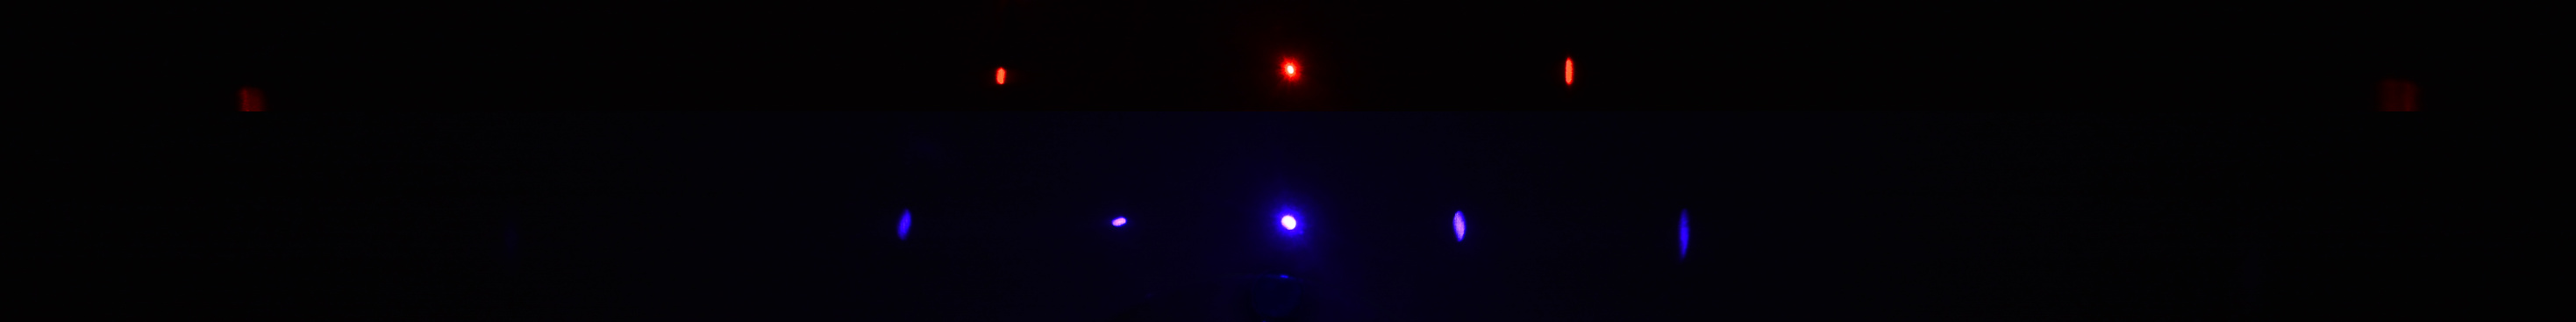
\includegraphics[width=140truemm]{slike/05_photos_CD.JPG}
\caption{Primer zelo velikega števila zelo tankih rež je zgoščenka (CD). Če z nje odstranimo
odbojno kovinsko plast, ostane prozorna plastična ploščica z vrezanim zapisom, na katerem se uklanja 
vpadna laserska svetloba. Različne valovne dolžine se uklanjajo pod različnimi koti, kar
da zgoščenkam značilen mavrični videz.}
\label{fig:05_uklon_cd}
\vglue-5truemm
\end{figure}
\begin{figure}[ht]
\centering
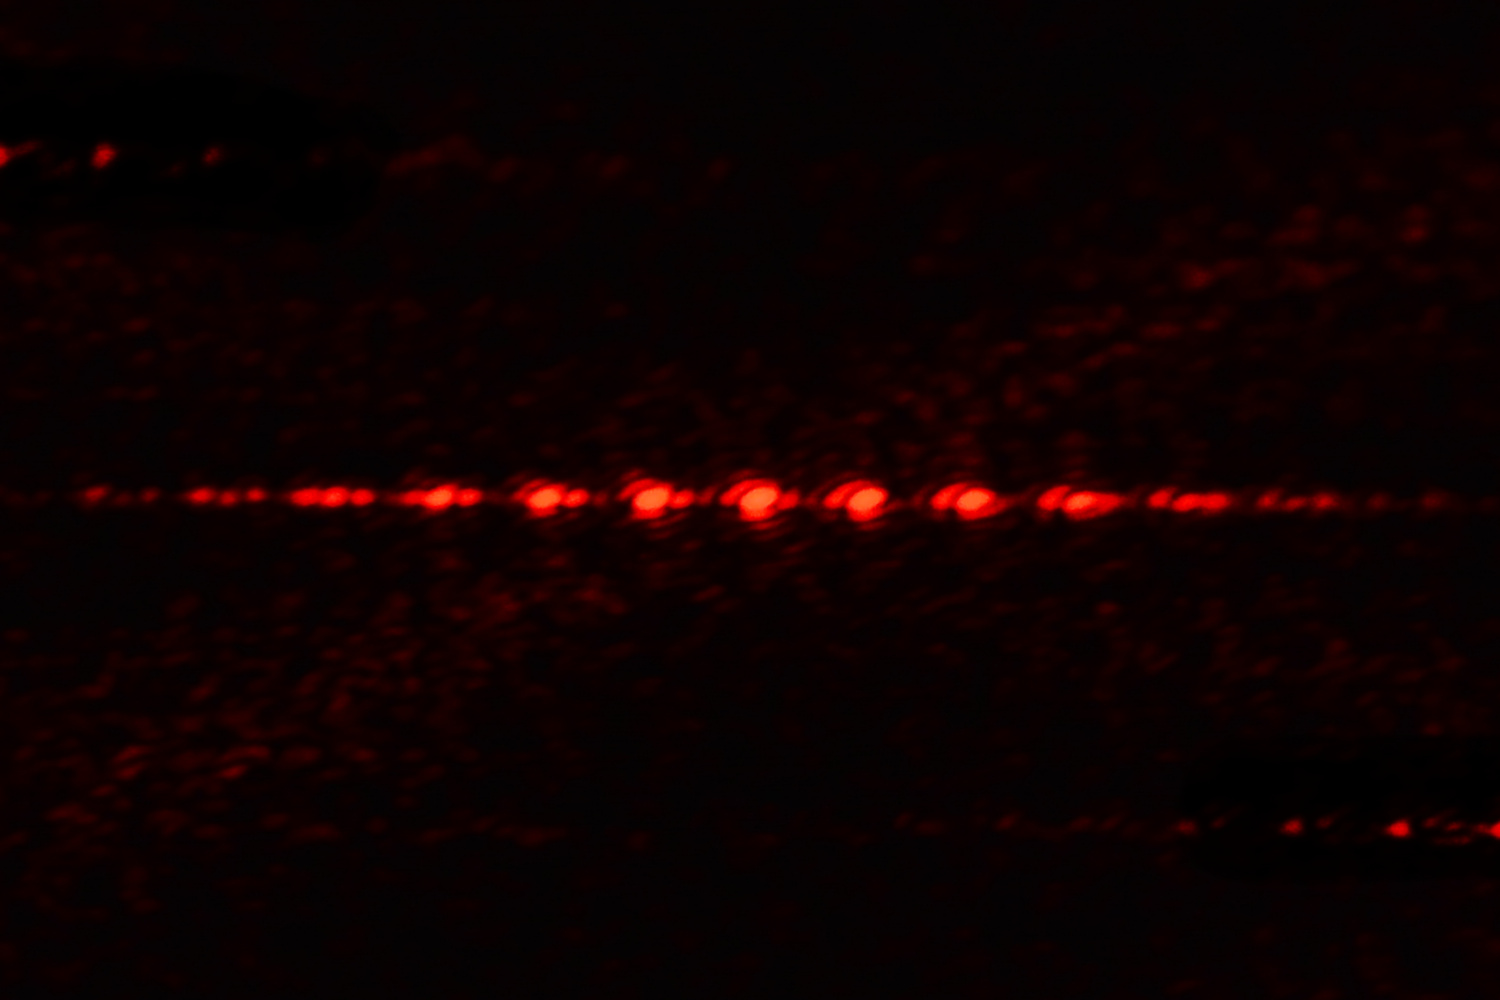
\includegraphics[width=70truemm]{slike/05_photos_perje.jpg}\hfill
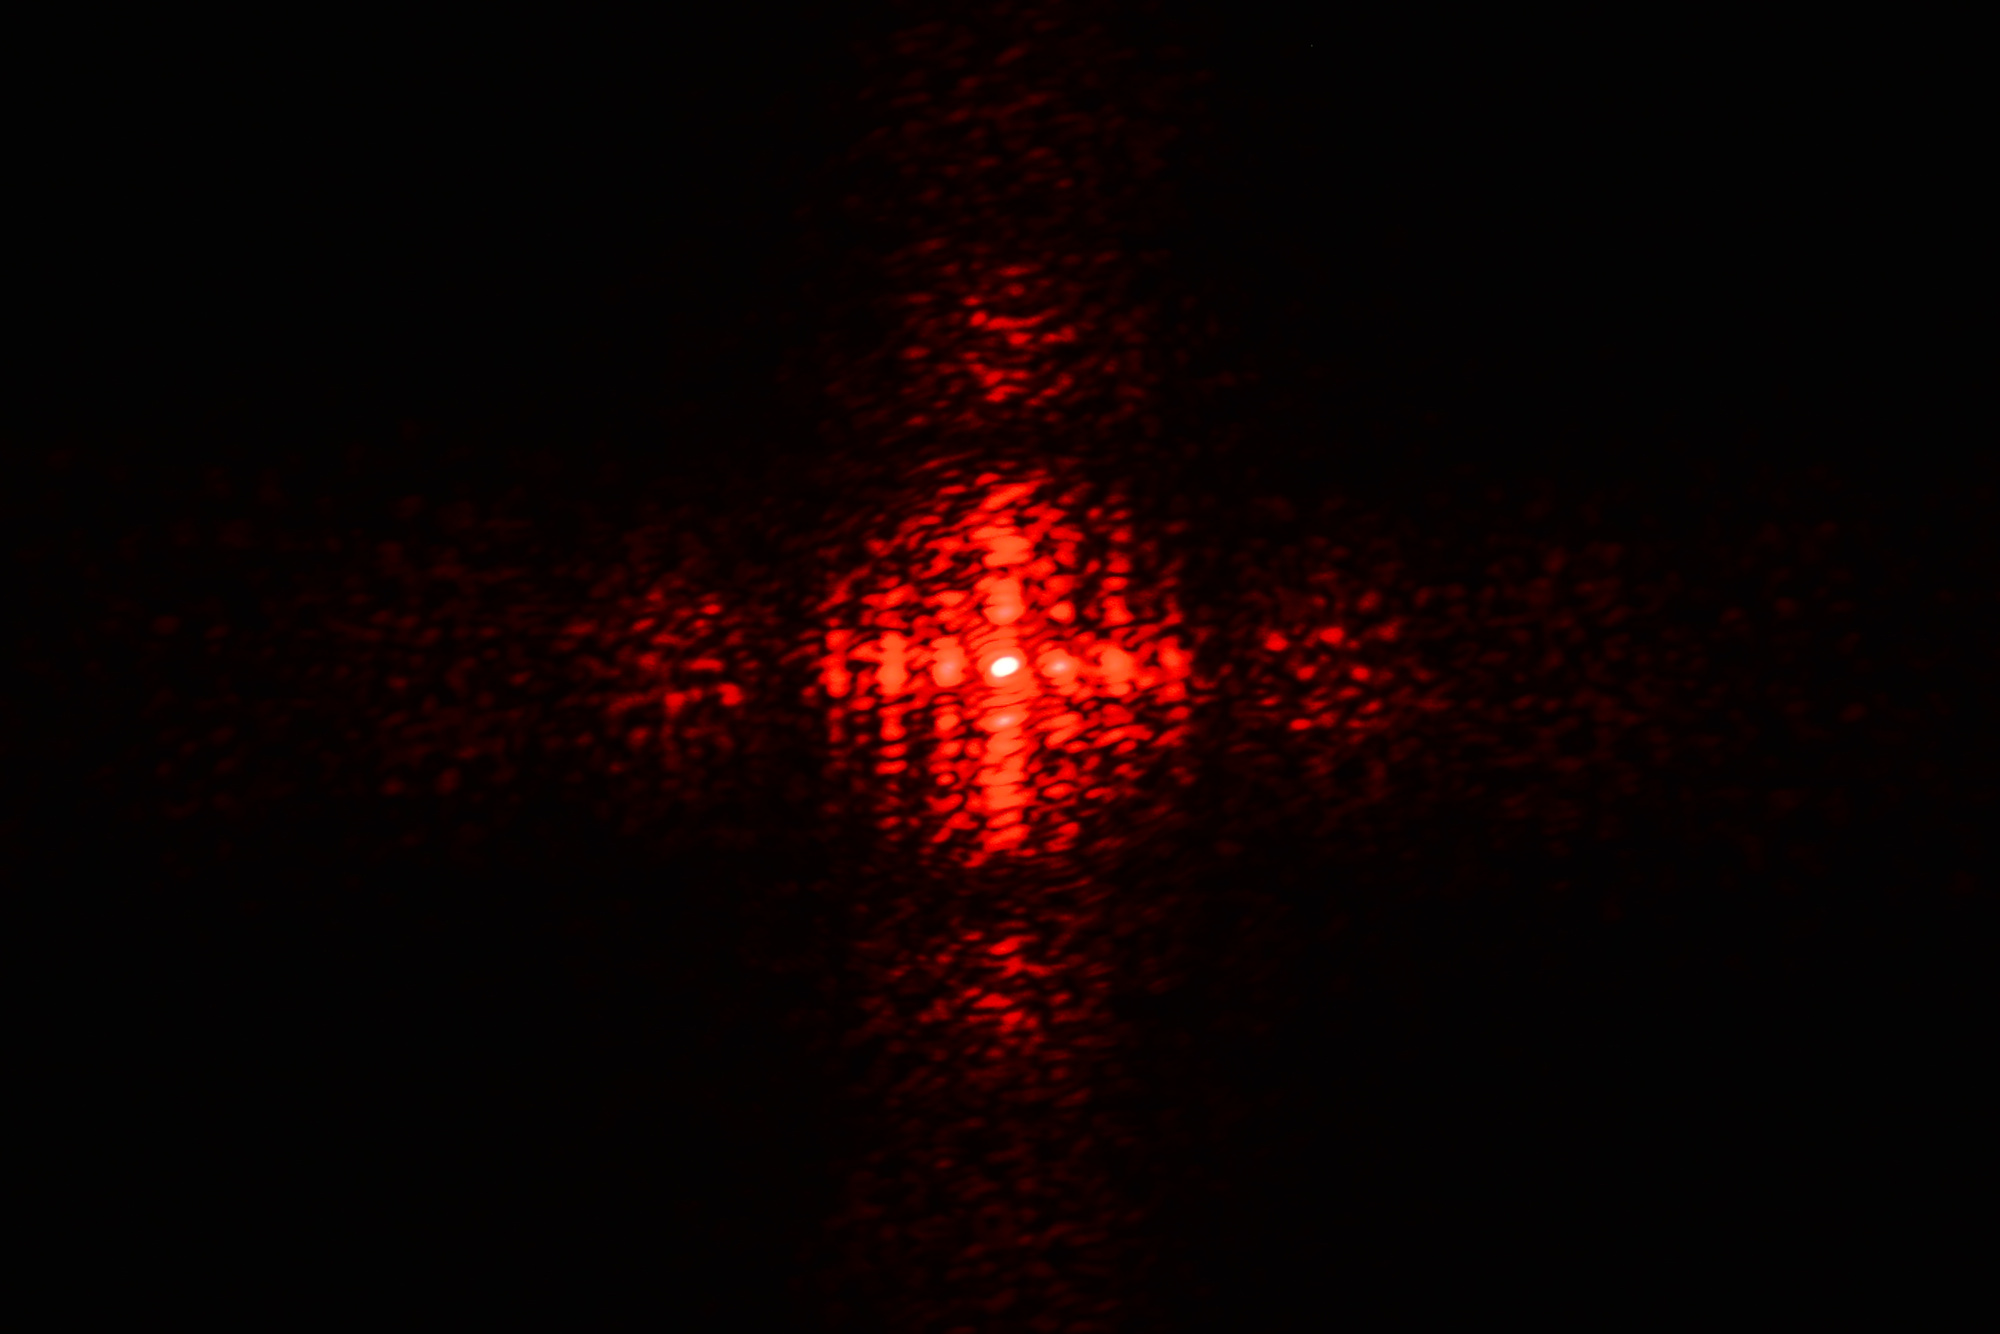
\includegraphics[width=70truemm]{slike/05_photos_ruta.jpg}
\caption{Uklon laserske svetlobe na ptičjem peresu (levo) in na gosto tkani svileni ruti (desno).
Dvodimenzionalna uklonska slika je produkt uklonskih slik v smereh $x$ in $y$.}
\label{fig:05_uklon_ruta}
\end{figure}
\vglue-5truemm
\end{example}

\begin{example}{\bf Fraunhoferjev uklon na okrogli odprtini s polmerom $a$.}
Kot naslednji primer si oglejmo Fraunhoferjev uklon na okrogli odprtini s polmerom $a$. 
Lego točke $P$ v objektni ravnini $xy$ opišemo v polarnih koordinatah $\varrho$ in $\varphi$
kot:
\beq
x = \varrho \cos \varphi \qquad \mathrm{in} \qquad y = \varrho \sin \varphi. 
\label{eq:05_30}
\eeq
Lego točke $P_0$ v opazovalni ravnini $\xi \eta$ zapišemo v polarnih koordinatah 
$q$ in $\phi$:
\beq
\xi = q \cos \phi \qquad \mathrm{in} \qquad \eta = q \sin \phi. 
\label{eq:05_31}
\eeq
\begin{figure}[ht]
\vglue-5truemm
\centering
\def\svgwidth{130truemm} 
\input{slike/05_koordinate_circ.pdf_tex}
\caption{Za izračun uklona na okrogli odprtini vpeljemo polarna koordinatna sistema 
($\varrho, \varphi$) na objektni ravnini in ($q, \phi$) na opazovalni ravnini.}
\label{fig:05_koordinate_circ}
\end{figure}

Uklonski integral (enačba~\ref{eq:Fraunhoferjev}) v novih koordinatah zapišemo kot:
\beq
E(q,\phi,z_0) = \frac{1}{i\lambda} \frac{E_0e^{ikR_0}}{R_0}\int_0^{2\pi} \int_0^a
e^{-i\omega_\xi x}e^{-i\omega_\eta y}\varrho d\varrho d\varphi.
\label{eq:05_32}
\eeq
Upoštevamo enačbe~(\ref{eq:05_13}, \ref{eq:05_14}, \ref{eq:05_30} in \ref{eq:05_31}) in zapišemo:
\beq
\omega_\xi x + \omega_\eta y= \frac{k}{R_0}q\cos \phi \varrho \cos\varphi + 
\frac{k}{R_0}q\sin \phi \varrho \sin\varphi = 
 \frac{k}{R_0} q\varrho\cos(\varphi - \phi).
\label{eq:05_33}
\eeq
Zaradi rotacijske simetrije lahko postavimo $\phi=0$ in zapišemo integral:
\beq
E(q,z_0) = \frac{1}{i\lambda} \frac{E_0e^{ikR_0}}{R_0}\int_0^{2\pi} \int_0^a
e^{-ikq\varrho \cos\varphi/R_0} \varrho d\varrho d\varphi.
\label{eq:05_34}
\eeq
Spomnimo se integralnega zapisa Besslove funkcije prve vrste ničtega reda:
\beq
J_0(u) = \frac{1}{2\pi} \int_0^{2\pi} e^{-iu\cos v }dv
\label{eq:05_35}
\eeq
in rekurzijske zveze:
\beq
\frac{d}{du}\left( u J_1(u)\right) = u J_{0}(u).
\label{eq:05_36}
\eeq
Primerjamo enačbi~(\ref{eq:05_34}) in (\ref{eq:05_35}) in vpeljemo
zvezi $v = \varphi$ in $u = kq\varrho/R_0$. Integriramo enačbo~(\ref{eq:05_34}) 
najprej po $\varphi$ z upoštevanjem enačbe~(\ref{eq:05_35}), nato še po $\varrho$
z upoštevanjem enačbe~(\ref{eq:05_36}). Dobimo:
\beq
E = \frac{1}{i\lambda}\frac{E_0 e^{ikR_0}}{R_0}~\pi a^2~\frac{2 J_1 (kqa/R_0)}{kqa/R_0}.
\label{eq:05_37}
\eeq
Vpeljemo uklonski kot $\vartheta \approx q/R_0$ in zapišemo gostoto svetlobnega toka
uklonjene svetlobe:
\boxeq{eq:uklonAiry}{
j = j_0 \left(\frac{2J_1(ka\sin\vartheta)}{ka\sin \vartheta}\right)^2\!\!.
}
Opisano uklonsko sliko imenujemo Airyjeva uklonska slika 
in osrednji krog Airyjev disk 
po angleškem matematiku in astronomu Siru Georgeu Biddellu Airyu (1801--1892). 
Uklonska slika je  po pričakovanju rotacijsko simetrična.  
\begin{figure}[ht]
\centering
\centering
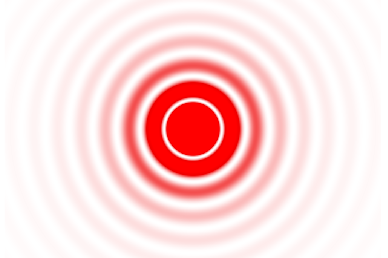
\includegraphics[width=7truecm]{slike/05_circ_sim.png}\hfill
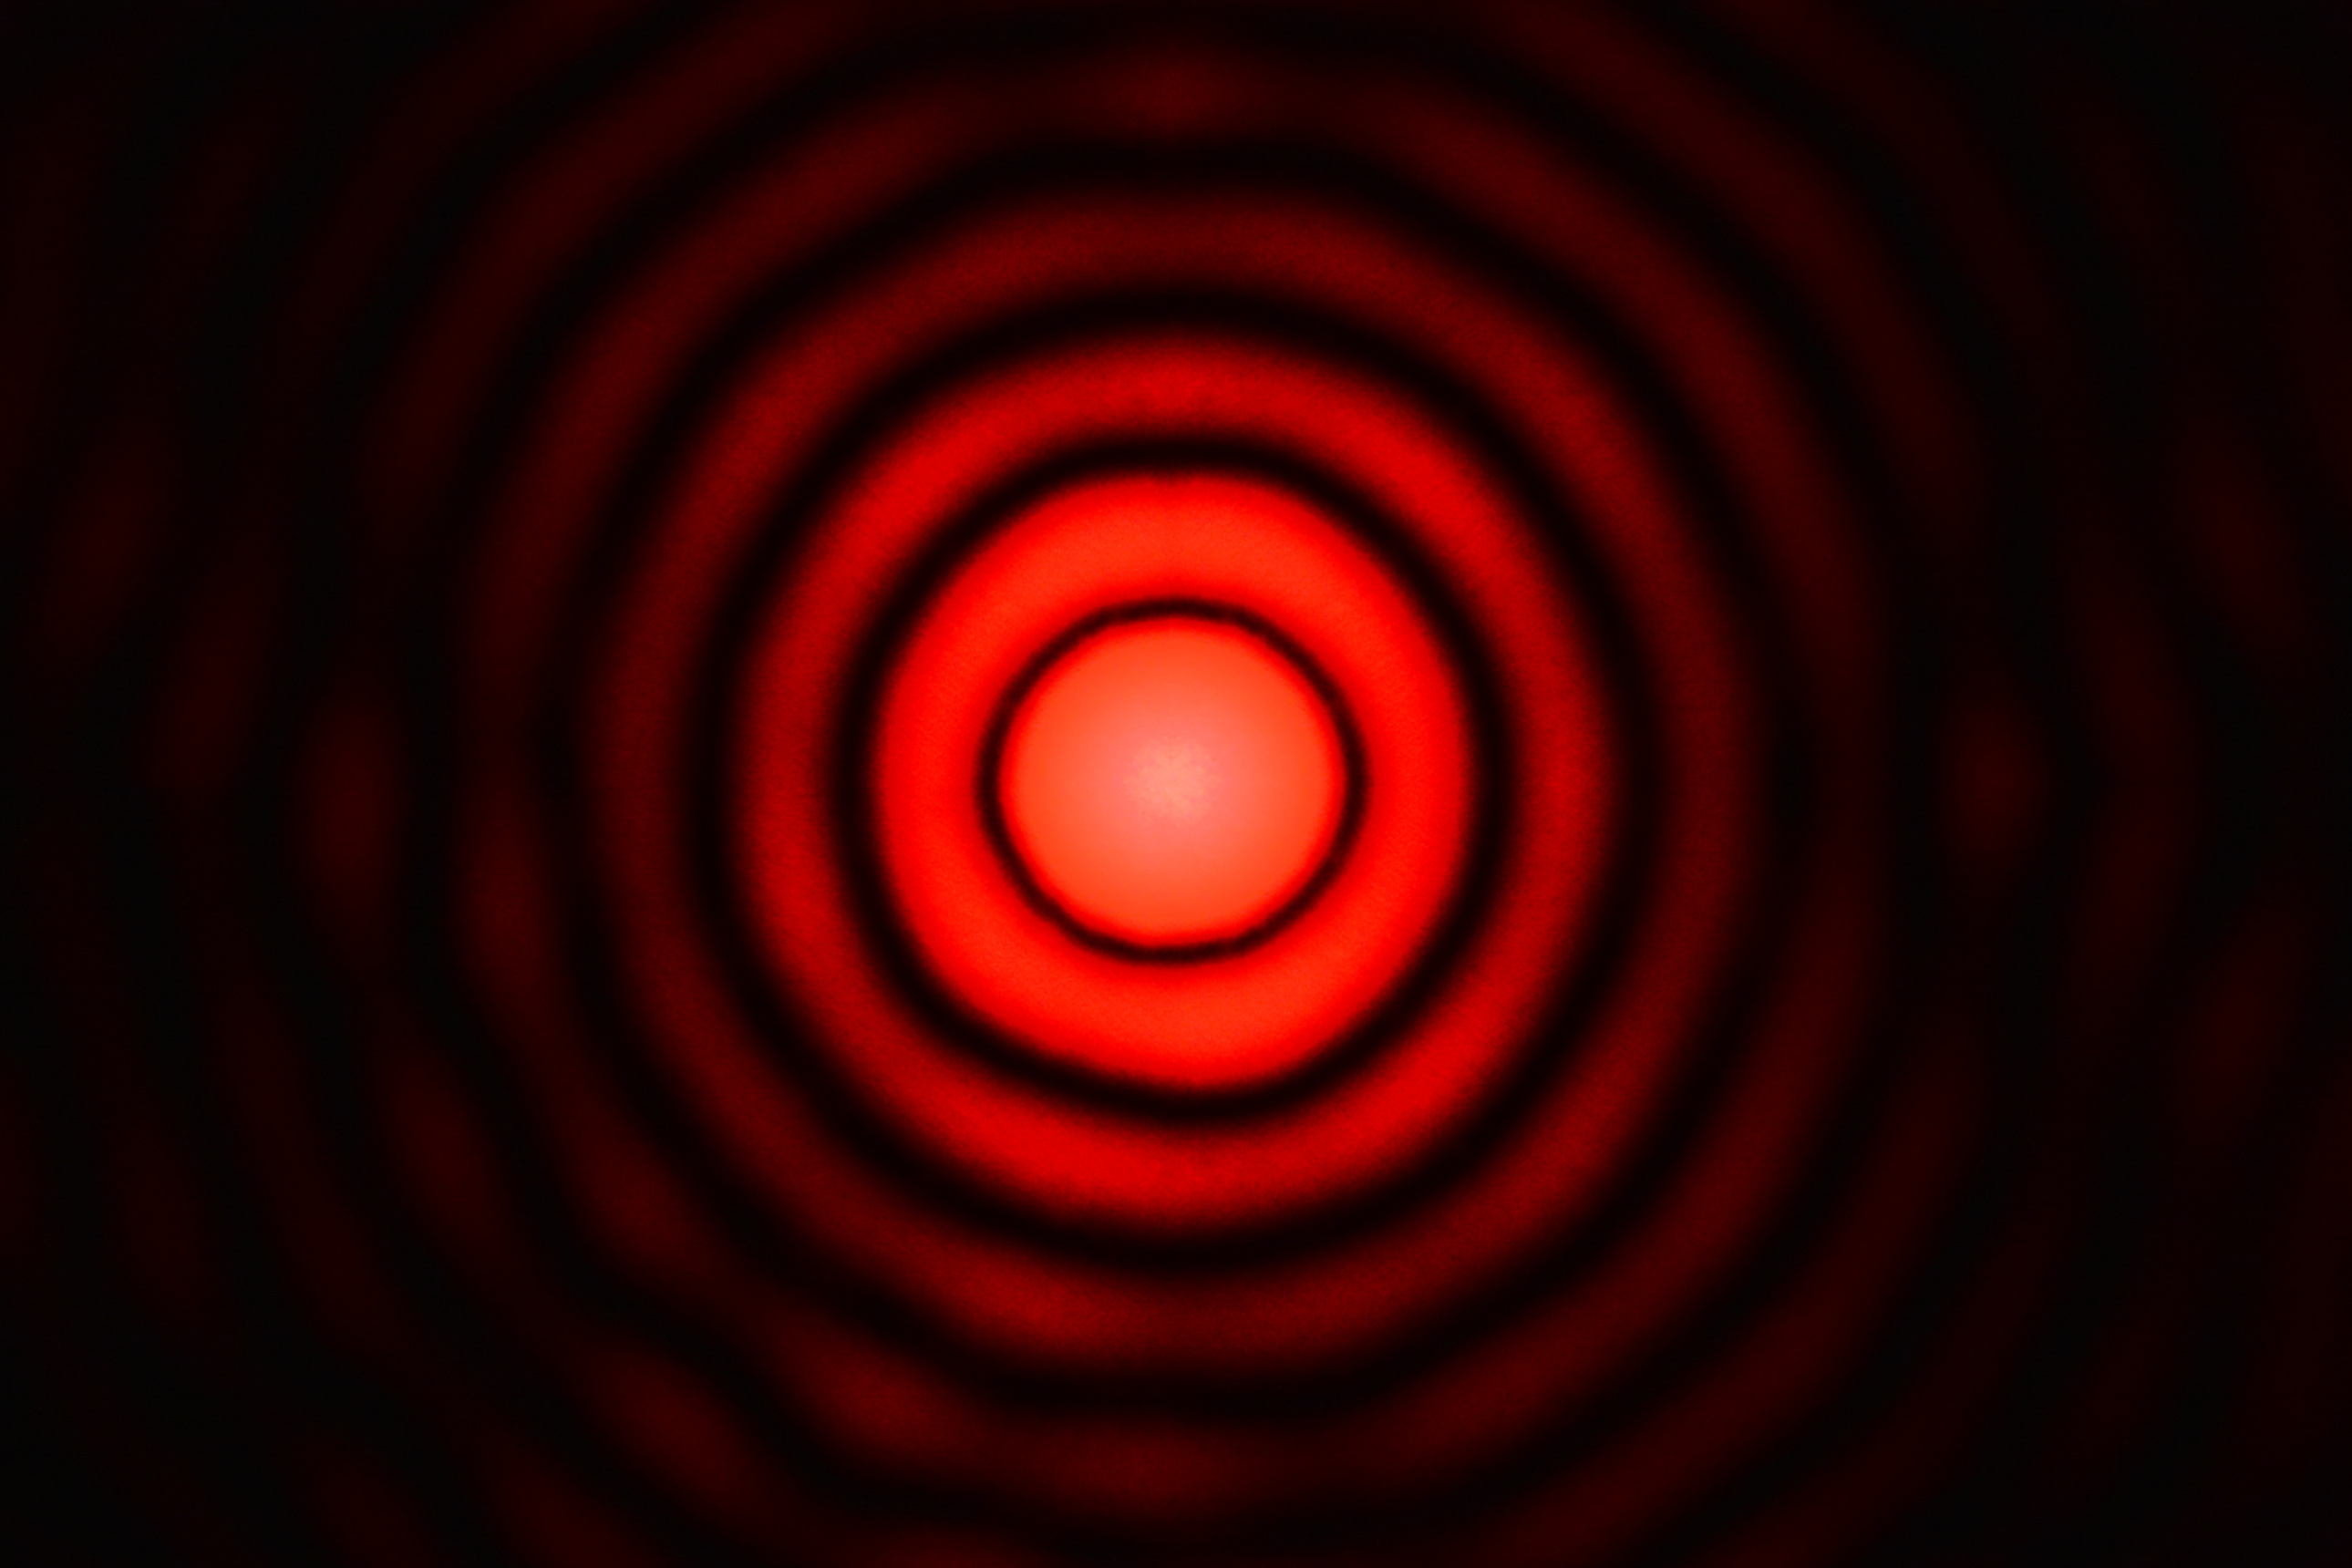
\includegraphics[width=7truecm]{slike/05_circ.JPG}
\caption{Simulacija Fraunhoferjeve uklonske slike na okrogli odprtini in fotografija
uklona na luknjici v papirju.}
\label{fig:05_Airy}
\end{figure}

V smeri naravnost (na sredini Airyjevega diska) 
je gostota svetlobnega toka enaka $j_0$, saj velja:
\beq
\lim_{u \to 0}\frac{J_1(u)}{u} = \frac{1}{2}.
\label{eq:05_39}
\eeq
Z naraščajočim uklonskim kotom intenziteta uklonjene svetlobe pojema, nato
spet naraste in ponovno pojema ... Ničle uklonske slike so določene
z ničlami Besslove funkcije in se pojavijo pri vrednostih:
\beq
ka\sin\vartheta  \approx 3,83;~7,02;~10,17;~13,32~...
\label{eq:05_40}
\eeq
Intenziteta stranskih obročev je razmeroma šibka, zato je najpomembnejši
notranji krog uklonske slike. Inteziteta prvega obroča je namreč le okoli $2~\%$ vršne
intenzitete, ostali obroči pa so še občutno šibkejši.

Polmer notranjega kroga (Airyjevega diska) $q_A$ izračunamo iz zveze:
\beq
ka\,q_A/R_0 = \frac{2\pi a}{\lambda}\frac{q_A}{R_0} = 3,83
\label{eq:05_41}
\eeq
in dobimo:
\beq
q_A = \frac{3,83}{\pi}\frac{\lambda R_0}{2a} = 1,22~\frac{\lambda R_0}{2a}.
\label{eq:05_42}
\eeq

Po Babinetovem načelu nastane enaka uklonska slika, če se svetloba uklanja
na okrogli odprtini v zaslonu ali na okroglem predmetu. Primer majhnih okroglih
predmetov, ki jih v velikem številu najdemo v naravi, so oblaki. Ko na primer svetloba
s Sonca ali z Lune vpada na plast drobnih kapljic v ozračju, se na njih uklanja in pojavi se
tako imenovana korona. Podoben pojav opazimo na zarošenem oknu. 
\begin{figure}[ht]
\centering
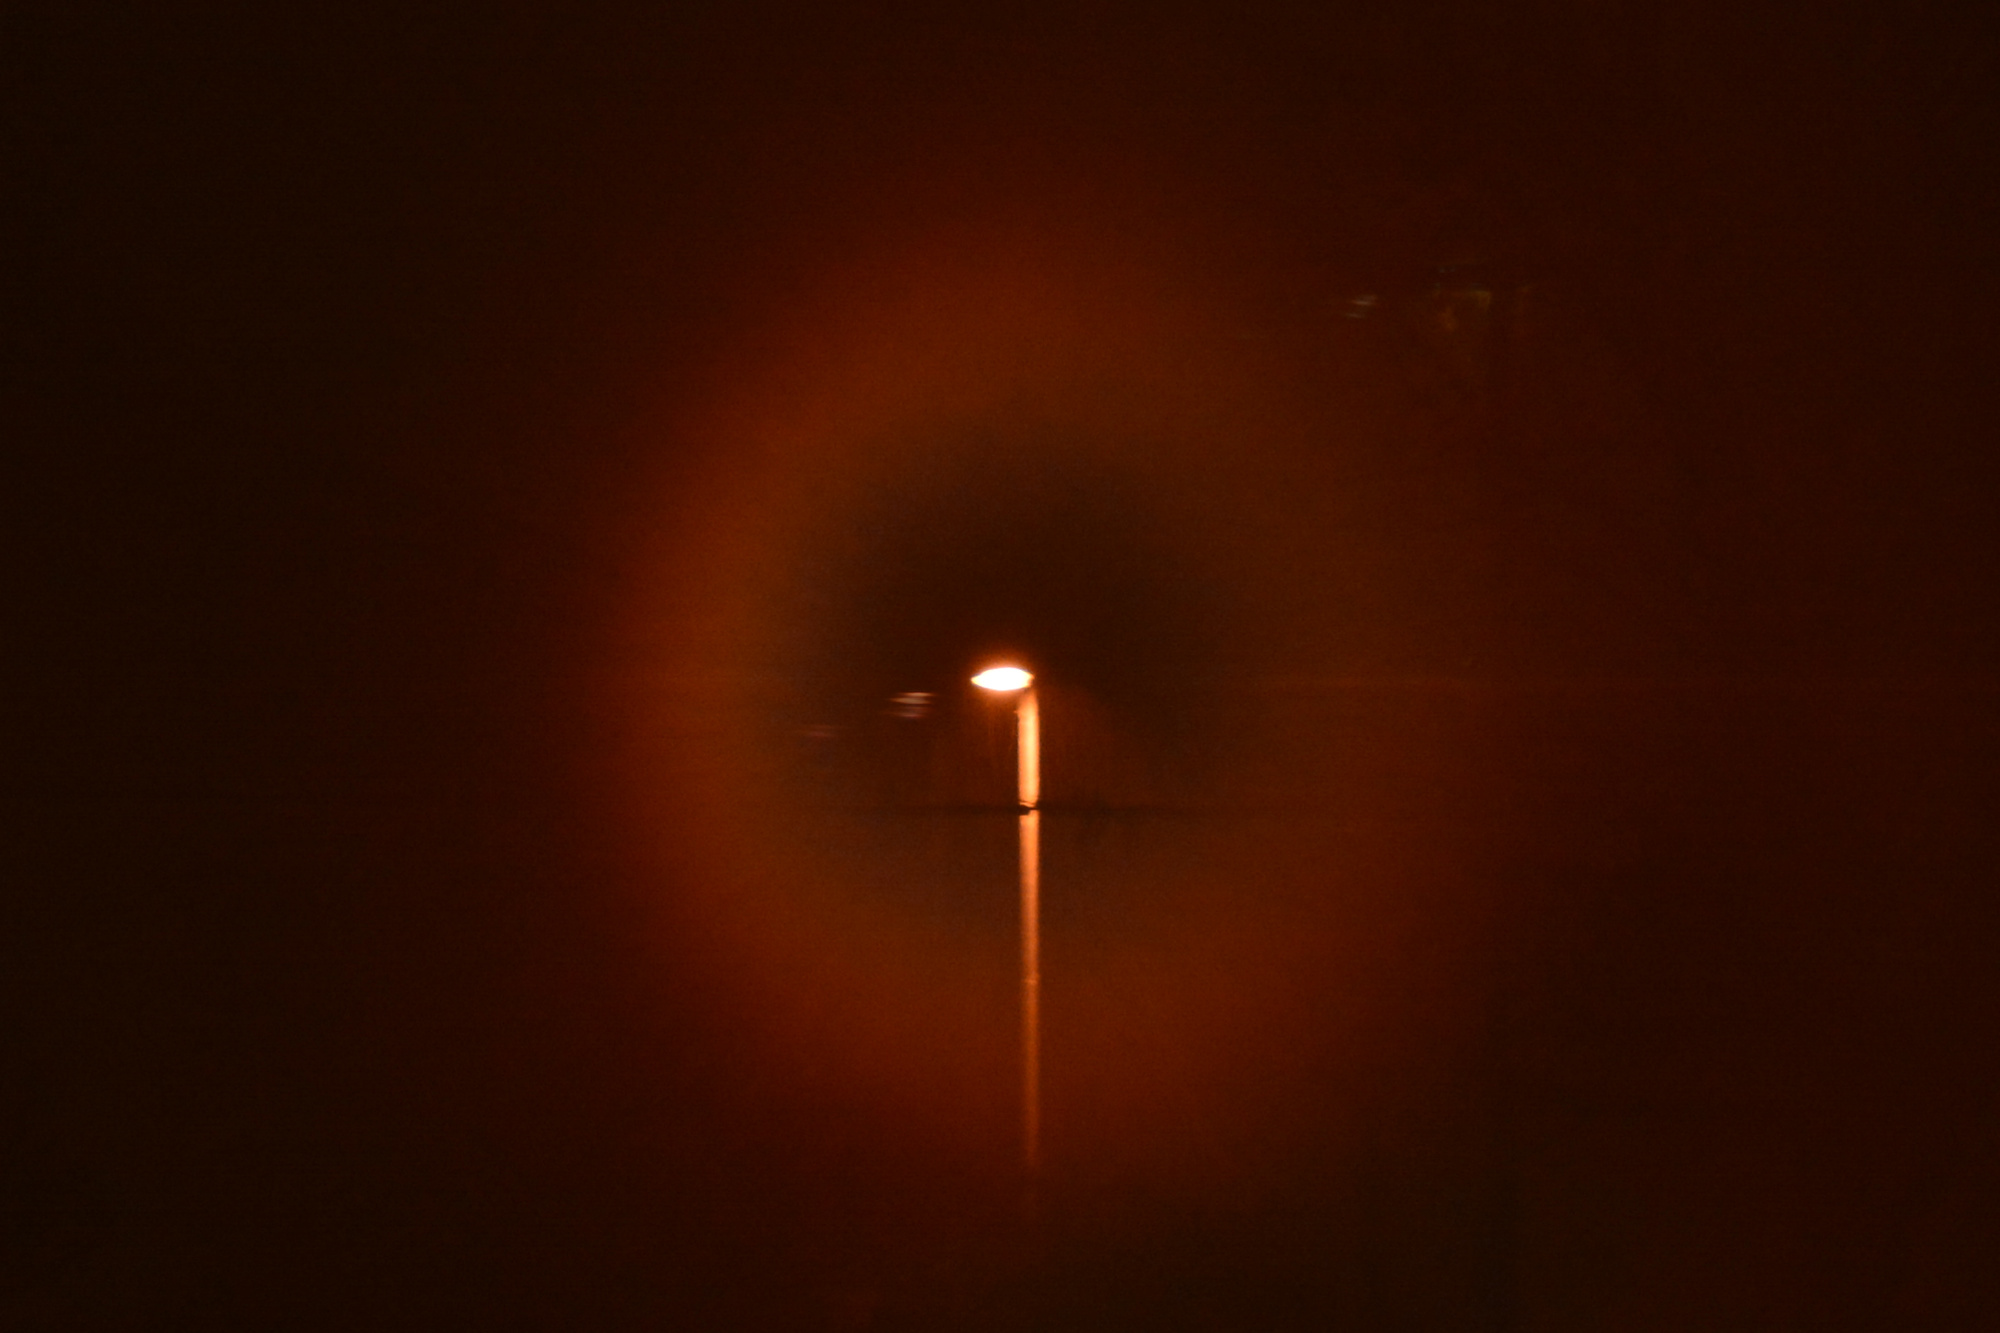
\includegraphics[width=70truemm]{slike/05_photos_svetilka.jpg}\hfill
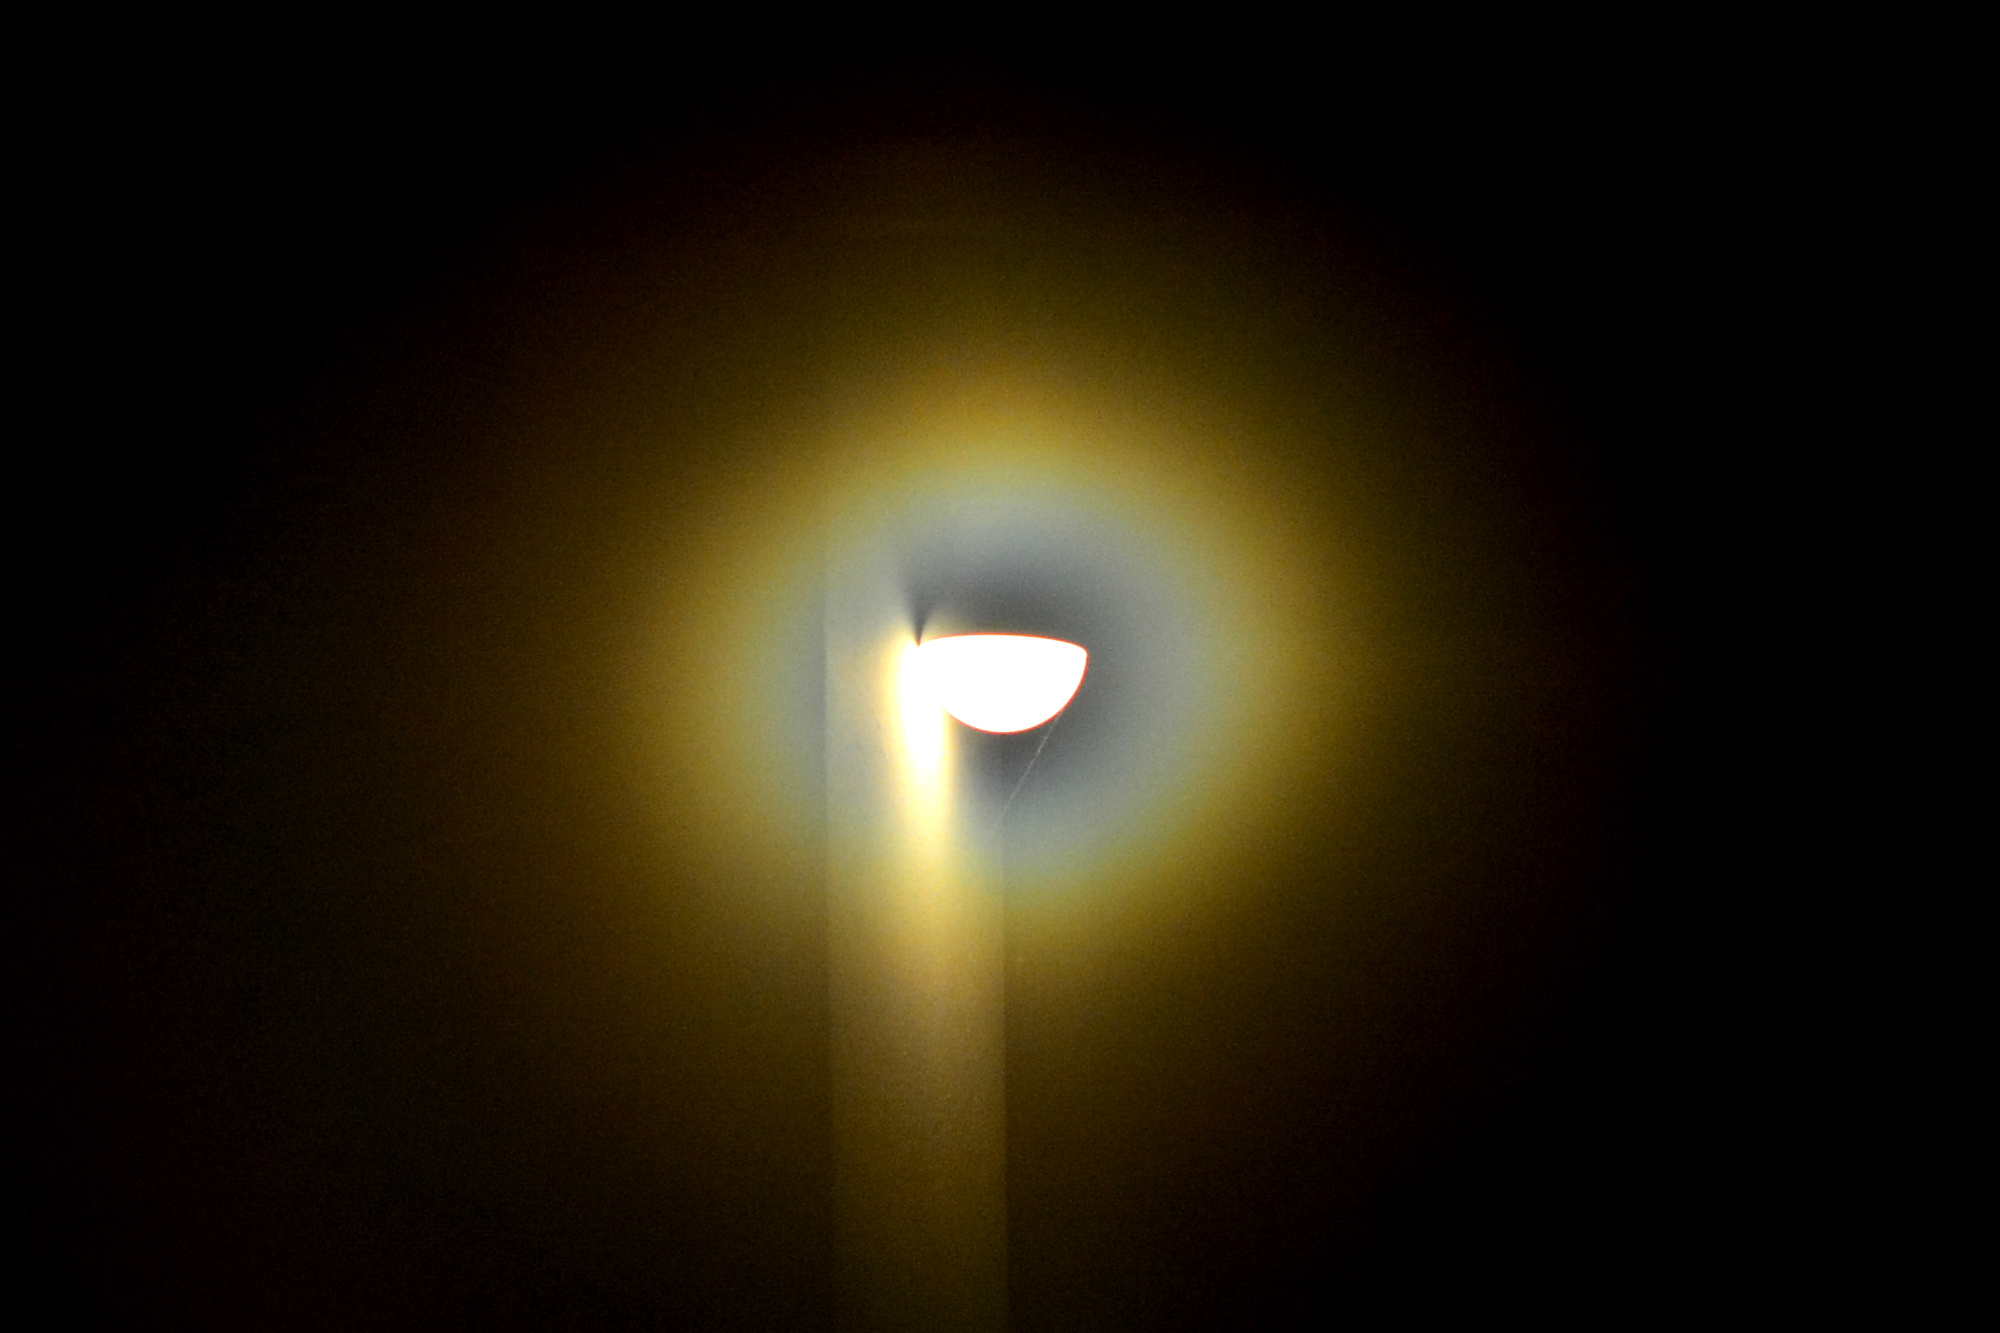
\includegraphics[width=70truemm]{slike/05_photos_luc.jpg}
\caption{Svetloba s svetilke se uklanja na drobnih kapljicah na zarošenem oknu (levo). Če je svetloba
bela, se različne barve uklanjajo pod različnimi koti in vidimo barvne obroče (desno).}
\label{fig:05_uklon_svetilka}
\end{figure}
\vglue-5truemm

\end{example}

\section{Ločljivost optičnih naprav}
Pri optičnih napravah (na primer mikroskopu ali daljnogledu) 
svetloba potuje skozi leče in nato vpade na svetlobni detektor. Leče pri tem delujejo
kot okrogle odprtine, na katerih se svetloba uklanja, kar omejuje ločljivost 
optičnih naprav.

Poglejmo najpreprostejši primer ene same leče z goriščno razdaljo $f$ in premerom $D$,
skozi katero opazujemo zelo oddaljen točkast predmet. Slika predmeta 
nastane v goriščni ravnini, zato je $R_0=f$. Zaradi uklona točkasti predmet na 
detektorju po enačbi~(\ref{eq:05_42}) vidimo kot okrogel disk s polmerom $q$:
\beq
q \approx q_A = 1,22~\frac{f\lambda}{D} = 1,22~\frac{\lambda}{D/f} = 0,61~\frac{\lambda}{NA},
\label{eq:05_43}
\eeq
pri čemer je numerična apertura $NA$ razmerje med polmerom leče $D/2$
in goriščno razdaljo $f$:
\beq
NA = \frac{D/2}{f}.
\label{eq:05_44}
\eeq
Značilne vrednosti za numerično aperturo so $NA \lesssim 1$.

Opazujmo dve oddaljeni točkasti telesi skozi lečo z numerično aperturo $NA$. 
V opazovalni ravnini vsako od njiju ustvari svoj Airyjev disk. Kadar se začneta osrednja
kroga uklonske slike med seboj prekrivati, teles na sliki ne moremo več ločiti. Kriterij, ki določa,
ali dva objekta na sliki še ločimo med seboj, imenujemo
Rayleighev kriterij ločljivosti po angleškemu fiziku Lordu Rayleighu (1842--1919). 
\begin{figure}[ht]
\centering
\def\svgwidth{120truemm} 
\input{slike/05_locljivost.pdf_tex}
\caption{Ko se uklonski sliki dveh točkastih predmetov prekrivata, ju ne moremo več ločiti.
Najmanjši kot $\alpha$, pri katerem predmeta še ločimo, določa ločljivost naprave.}
\label{fig:05_locljivost}
\end{figure}

\begin{figure}[ht]
\centering
\def\svgwidth{120truemm} 
\input{slike/05_locljivost2.pdf_tex}
\caption{Po Rayleighevem kriteriju sliki dveh teles ločimo, če je razdalja med
njunima središčema večja (levo) ali enaka polmeru Airyjevega diska (sredina). Če 
sta sliki teles bliže, ju ne ločimo (desno).}
\label{fig:05_locljivost2}
\end{figure}

Rayleighev kriterij pravi, da objekta ločimo, če velja:
\beq
\alpha \ge \alpha_{\mathrm{min}} = 
\frac{q_{A}}{f} = 1,22~\frac{\lambda}{D}.
\label{eq:05_46}
\eeq
Manjši minimalni zorni kot in s tem večjo kotno 
ločljivost optičnih naprav, na primer teleskopov, torej
dosežemo pri manjših valovnih dolžinah svetlobe in večjih lečah.

Na podoben način izračunamo tudi ločljivost optičnih mikroskopov. Ker
je pri mikroskopih predmet blizu goriščne razdalje, je najmanjši 
razmik med točkama, ki ju še ločeno opazujemo, enak:
\beq
d_\mathrm{min} = \alpha_{\mathrm{min}} f = 1,22~\frac{\lambda f}{D} = 
0,61~\frac{\lambda}{NA} \sim \lambda.
\label{eq:05_46aa}
\eeq
Ločljivost mikroskopov je tako približno enaka 
valovni dolžini svetlobe, s katero opazujemo predmet: 
$d_\mathrm{min} \sim \lambda$.

\begin{remark}
Ločljivost optičnih naprav izboljšamo z uporabo krajše valovne dolžine svetlobe.
Z modro svetlobo tako lahko opazujemo manjše predmete
kot z rdečo. Uporaba krajše valovne dolžine med drugim omogoča zgostitev 
zapisa na zgoščenkah. Z navadne zgoščenke (CD) beremo podatke z valovno 
dolžino $780~\si{\nano\metre}$, z zgoščenke DVD z valovno dolžino
$650~\si{\nano\metre}$ in z Blu-ray plošč s svetlobo z valovno dolžino
$405~\si{\nano\metre}$, kar omogoča gostejši zapis večje količine podatkov.
Dodatno se pri novejših tehnologijah uporablja lečo z večjo numerično
aperturo, kar zmanjša polmer laserske pike
z $800~\si{\nano\metre}$ na $250~\si{\nano\metre}$.
\end{remark}

\begin{example}{\bf Ločljivost teleskopa.}
S teleskopom, ki ima lečo s premerom $D=5~\si{m}$,
opazujemo Luno, ki je od Zemlje oddaljena $L = 384\,000~\si{km}$. 
Ocenimo velikost podrobnosti na Luninem površju, ki jih še ločimo
s svetlobo z valovno dolžino $500~\si{nm}$. 

Iz enačbe~(\ref{eq:05_46}) ocenimo:
\beq
d_\mathrm{min} = 1,22~\frac{\lambda}{D} L \approx 50~\si{m}.
\label{eq:05_47}
\eeq
\end{example}

\section{Fresnelov uklon}
Doslej smo predpostavili, da je optično polje, ki vpada na objektni zaslon $xy$, povsod 
konstantno in enako $E_0$ (slika~\ref{fig:05_shema}). 
Obravnavajmo zdaj primer, ko je svetloba, 
ki vpada na objektni zaslon, funkcija kraja $E_0 = E_0(x,y)$. 

Naj izvor svetlobe $S$, ki oddaja krogelno valovanje, leži v ravnini 
$x'y'$. Razdalja med ravnino izvora svetlobe in objektno ravnino
naj bo enaka $z_0'$ (slika~\ref{fig:05_Fresnel}).
\begin{figure}[ht]
\centering
\def\svgwidth{120truemm} 
\input{slike/05_Fresnel_koor.pdf_tex}
\caption{Svetloba izvira iz točke $S$ v ravnini $x'y'$ in vpada na objektno ravnino $xy$ na 
oddaljenosti $z_0'$. V opazovalni ravnini $\xi\eta$ opazujemo uklonsko
sliko odprtine oziroma predmeta.}
\label{fig:05_Fresnel}
\vglue-3truemm
\end{figure}

Polje v točki $P$ v objektni ravnini zapišemo kot 
\beq
E_0 (x,y,0) = \tilde{E}_0 \frac{e^{ikR'}}{R'}.
\label{eq:05_65}
\eeq
Uklonski integral (enačba~\ref{eq:05_05}) se potem zapiše kot:
\beq
E(\xi, \eta, z_0) = \frac{1}{i\lambda} \tilde{E}_0 \int_{-\infty}^{\infty}
\int_{-\infty}^{\infty} f(x,y)~\frac{e^{ikR'}}{R'}~\frac{e^{ikR}}{R}~dx\,dy.
\label{eq:05_66}
\eeq
Izraz za $R$ razvijemo v Taylorjevo vrsto (enačba~\ref{eq:05_10}) in dobimo:
\beq
R\approx R_0 - \frac{\xi x}{R_0} - \frac{\eta y}{R_0} + \frac{x^2+y^2}{2R_0} + ...
\label{eq:05_67}
\eeq
Pri Fraunhoferjevem uklonu smo upoštevali prve tri člene v razvoju, 
četrtega, kvad\-rat\-ne\-ga pa smo zanemarili. V Fresnelovem uklonskem 
približku upoštevamo tudi kvadratni člen. 

Zapišimo razdaljo $R$ drugače:
\beq
R  = \sqrt{z_0^2 + (x-\xi)^2 + (y-\eta)^2} \approx z_0 + \frac{(x-\xi)^2+(y-\eta)^2}{2z_0}
\label{eq:05_75a}
\eeq
in podobno $R'$:
\beq
R'  = \sqrt{z_0'^2 + (x-x')^2 + (y-y')^2} \approx z_0' + \frac{(x-x')^2+(y-y')^2}{2z_0'}.
\label{eq:05_75}
\eeq
Razvoja vstavimo v uklonski integral (enačba~\ref{eq:05_66}) in dobimo Fresnelov uklonski približek:
\boxeq{eq:Fresnel}{
E(\xi, \eta, z_0) = \frac{1}{i\lambda} \frac{\tilde{E}_0 e^{ik(z_0'+z_0)}}{z_0'\,z_0} 
\int\!\!\!\!\!\int_{-\infty}^{\infty} f(x,y)\,e^{\frac{ik}{2z_0'}((x-x')^2+(y-y')^2)} 
e^{\frac{ik}{2z_0}((x-\xi)^2+(y-\eta)^2)}\, dx\,dy.
}
Pri tem smo $R$ in $R'$ v imenovalcu ulomka 
nadomestili z $z_0$ in $z_0'$ in ju postavili 
pred integral, saj je odvisnost razmeroma šibka.

Zapisani izraz Fresnelovega uklona (enačba~\ref{eq:Fresnel}) je za analitično 
računanje precej zahtevnejši od Fraunhoferjevega uklona 
(enačba~\ref{eq:Fraunhofer}), zato bomo obravnavali
le dva primera: Fresnelove conske plošče in uklon na pravokotni reži oziroma ostrem robu. Preden se lotimo primerov, poglejmo še veljavnost Fresnelovega približka.

Izhajamo iz enačbe~(\ref{eq:05_75a}) in 
vpeljemo parameter $d^2 = (x-\xi)^2+(y-\eta)^2$. Potem velja:
\beq
R \approx z_0 + \frac{1}{2}\frac{d^2}{z_0} - \frac{1}{8}\frac{d^4}{z_0^3} + ...
\label{eq:05_69}
\eeq
V Fresnelovem približku smo obdržali prva dva člena, višje člene pa 
smo zanemarili. To lahko naredimo, če za vse vrednosti $x$ in $y$ v odprtini velja:
\beq
k\left( \frac{1}{8}\frac{d^4}{z_0^3}\right) \ll 2\pi.
\label{eq:05_70}
\eeq
Pogoj preoblikujemo v:
\beq
\left(\frac{d}{z_0}\right)^4 \ll \frac{8\lambda}{z_0}.
\label{eq:05_71}
\eeq
Fresnelov približek je veljaven, kadar je izpolnjen zgornji pogoj.
\begin{example}{\bf Veljavnost Fresnelovega približka.}
Naj na odprtino s polmerom $d=1~\si{mm}$ vpada svetloba
z valovno dolžino $500~\si{nm}$. Izračunajmo oddaljenost
od zaslona $z_0$, pri kateri je izpolnjen pogoj za Fresnelov
uklonski približek. Iz enačbe~(\ref{eq:05_71}) sledi:
\beq
z_0\gg \sqrt[3]{d^4/8\lambda} \approx 6~\si{mm}.
\label{eq:05_73}
\eeq
Spomnimo se, da je pogoj za veljavnost Fraunhoferjevega
približka (Primer~\ref{ex:fh}) pri enakem polmeru odprtine 
$z_0 \gg 2~\si{\metre}$. 
Izračunajmo še Fresnelovo število (enačba~\ref{eq:05_17})
za $z_0=6~\si{mm}$:
\beq
F = \frac{d^2}{\lambda R_0} \approx 300. 
\label{eq:05_74}
\eeq
Fresnelovo število $F\gg1$, kar potrjuje veljavnost Fresnelovega približka.
\end{example}

\begin{example}{\bf Fresnelova conska plošča.}
Izračunajmo najpreprostejši primer Fresnelovega uklona na 
okrogli odprtini s polmerom $a$. Točkasti izvor svetlobe naj leži na 
optični osi $z$, ki je hkrati simetrala odprtine, na 
razdalji $z_0'$ pred odprtino. Opazujemo uklon
na optični osi na oddaljenosti $z_0$ za odprtino (slika~\ref{fig:05_FresCona}).
\begin{figure}[ht]
\centering
\def\svgwidth{100truemm} 
\input{slike/05_FresCona.pdf_tex}
\caption{K računu Fresnelovega uklona, ko izvor in 
detektor ležita na osi okrogle odprtine}
\label{fig:05_FresCona}
\end{figure}

Izhajamo iz enačbe za Fresnelov uklon~(\ref{eq:Fresnel}) in vstavimo 
$x'=y'=0$ in $\xi = \eta = 0$. Dobimo:
\beq
E(0,0, z_0) = \frac{1}{i\lambda} \frac{\tilde{E}_0 
e^{ikz_0'+ikz_0}}{z_0'z_0} \int_{-\infty}^{\infty}
\int_{-\infty}^{\infty} f(x,y)\,
e^{\frac{ik}{2z_0'}(x^2+y^2)} e^{\frac{ik}{2z_0}(x^2+y^2)} dx\, dy.
\label{eq:05_77}
\eeq
Zaradi rotacijske simetrije računamo v cilindričnih koordinatah in 
vpeljemo $\varrho = \sqrt{x^2 + y^2}$ ter $dx\,dy = \varrho d\varrho d\varphi$,
pri čemer je $\varphi$ polarni kot. Aperturna funkcija $f=1$ 
za $\varrho \leq a$, sicer velja $f= 0$. Integriramo po kotu $\varphi$ 
in dobimo:
\beq
E(0,0, z_0) = \frac{2\pi }{i\lambda} \frac{\tilde{E}_0 e^{ikz_0'+ikz_0}}{z_0'z_0} \int_{0}^{a}
e^{\frac{ik\varrho^2}{2}\left(\frac{1}{z_0'}+\frac{1}{z_0}\right)}\varrho d\varrho.
\label{eq:05_79}
\eeq
Vpeljemo:
\beq
\frac{1}{L} = \frac{1}{z_0'} + \frac{1}{z_0} \qquad \mathrm{in~~izrazimo} \qquad z_0'z_0 = L(z_0'+z_0).
\label{eq:05_80}
\eeq
Izračunamo še integral:
\beq
\int_0^a e^{ik\varrho^2/2L}\varrho d\varrho = \frac{L}{ik}\left(e^{ika^2/2L}-1\right) = 
\frac{2L}{k}e^{ika^2/4L} \sin\left(\frac{ka^2}{4L}\right)
\label{eq:05_81}
\eeq
in zapišemo jakost električnega polja:
\beq
E(0,0, z_0) = \frac{2\pi}{i\lambda} \frac{\tilde{E}_0 e^{ik(z_0'+z_0)}}{L(z_0'+z_0)} 
\frac{2L}{k}e^{ika^2/4L} \sin\left(\frac{ka^2}{4L}\right)\!\!.
\label{eq:05_81a}
\eeq
Gostota energijskega toka uklonjene svetlobe v točki $P_0$ je potem:
\boxeq{eq:05_82}{
j = 4 j_0 \sin^2\left(\frac{ka^2}{4L}\right)\!\!,
}
pri čemer $j_0$ označuje gostoto toka, kakršna bi bila na mestu opazovanja, 
če ne bi bilo zaslona:
\beq
j_0 = \frac{1}{2}\varepsilon_0 c \frac{\tilde{E}_0^2}{(z_0'+z_0)^2}.
\label{eq:05_83}
\eeq
Odvisnost gostote svetlobnega toka v točki $P_0$ od polmera odprtine
$a$ je prikazana na sliki~\ref{fig:05_FresCona2}. 
\begin{figure}[ht]
\centering
\def\svgwidth{90truemm} 
\input{slike/05_Fresnel_fcja.pdf_tex}
\caption{Odvisnost gostote svetlobnega toka $j$ na danem mestu v odvisnosti od polmera
okrogle odprtine $a$, na kateri se svetloba uklanja. Gostoto toka merimo glede na
gostoto toka $j_0$, ki bi bila na istem mestu, če ovire ne bi bilo. Polmeri $a_N$ označujejo
polmere posameznih Fresnelovih con.}
\label{fig:05_FresCona2}
\end{figure}

Največja vrednost, ki jo doseže $j$, je štirikratnik intenzitete $j_0$. Prvič to 
vrednost doseže pri polmeru $a_1$, ki ga imenujemo polmer
prve Fresnelove cone. Izračunamo ga iz pogoja:
\beq
\frac{ka_1^2}{4L} = \frac{\pi}{2}\qquad \mathrm{in} \qquad a_1  = \sqrt{\lambda L}.
\label{eq:05_84a}
\eeq
Z naraščajočim polmerom intenziteta gostota svetlobnega toka pojema do minimuma, 
ki ga doseže pri vrednosti $a_2$. Zanj velja:
\beq
\frac{ka_2^2}{4L} = \pi \qquad \mathrm{in} \qquad a_2 = \sqrt{2\lambda L}.
\eeq
Kolobar z notranjim polmerom $a_1$ in zunanjim polmerom 
$a_2$ imenujemo druga Fresnelova cona. 
Na splošno je $N$-ta Fresnelova cona kolobar, ki ga omejujeta polmera $a_{N-1}$ in $a_N$:
\beq
a_{N-1} = \sqrt{(N-1)\lambda L} < a < a_{N} = \sqrt{N \lambda L}.
\label{eq:05_90}
\eeq
V zaporednih kolobarjih gostota svetlobnega toka izmenično narašča in pojema. Razlike med
polmeri kolobarjev so vedno manjše, njihove ploščine pa so enake.
\vglue-3truemm
\begin{remark}
Oscilirajočo odvisnost intenzitete dobimo tudi, če namesto polmera odprtine 
spreminjamo lego točke $P_0$. Argument funkcije $\sin$ namreč prek parametra $L$
vsebuje koordinato $z_0$. S spreminjanjem lege opazovalne točke vzdolž optične osi
se tako na osi izmenično pojavljajo ojačitve in oslabitve. Na splošno velja, da se 
Fresnelova uklonska slika spreminja z oddaljenostjo od zaslona.
\end{remark}

Poglejmo podrobneje faze žarkov, ki izhajajo iz odprtine. Omejimo se
na primer $z_0' \to \infty$ oziroma $L = z_0$. Potem za žarke, ki so v 
odprtini od optične osi oddaljeni za $a$, velja (slika~\ref{fig:05_FresCona3}):
\beq
R^2 = z_0^2 + a^2.
\label{eq:05_85}
\eeq
Fazna zakasnitev takega valovanja v točki $P_0$ je:
\beq
\phi_a = kR = k\sqrt{z_0^2+a^2}.
\label{eq:05_86}
\eeq
fazna zakasnitev valovanja iz sredine cone pa je:
\beq
\phi_0 = kz_0.
\label{eq:05_87}
\eeq
Fazna razlika med valovanjem iz točke na oddaljenosti $a$ in valovanjem 
iz sredine je enaka:
\beq
\Delta \phi = \phi_a - \phi_0 = k\sqrt{z_0^2+a^2} - kz_0 \approx kz_0 + k \frac{a^2}{2z_0} - kz_0 = \frac{ka^2}{2z_0}.
\label{eq:05_87b}
\eeq
\begin{figure}[ht]
\centering
\def\svgwidth{120truemm} 
\input{slike/05_FresFaza.pdf_tex}
\caption{Pot, ki jo prepotuje valovanje od točke na razdalji $a$ do točke $P_0$, je enaka $R$ (levo).
Prispevki sekundarnih polj se seštevajo za $\Delta \phi < \pi$,  pri večjih fazni razlikah
se začnejo prispevki odštevati in skupno polje zmanjševati (sredina).}
\label{fig:05_FresCona3}
\vglue-5truemm
\end{figure}

Dokler je razlika faz manjša od $\pi$, se prispevki sekundarnih krogelnih valov iz odprtine k jakosti
električnega polja seštevajo, saj imajo vsi isti predznak (slika~\ref{fig:05_FresCona3}). Pri valovanjih,
katerih fazni zamik se od osrednjega razlikuje za več kot za $\pi$, kaže jakost električnega polja
v nasprotno smer in celotno polje se zmanjšuje. Največja intenziteta svetlobe je tako dosežena pri 
$\Delta \phi = \pi$. Velja:
\beq
\frac{ka_\mathrm{max}^2}{2z_0} = \pi \qquad \mathrm{in} \qquad a_\mathrm{max} = 
\sqrt{\frac{2\pi z_0}{k}} = \sqrt{z_0 \lambda}. 
\label{eq:05_87c}
\eeq
Izračunana vrednost polmera, do katerega intenziteta svetlobe na danem mestu narašča, je po pričakovanju enaka 
polmeru prve Fresnelove cone $a_\mathrm{max} = a_1$.  
Če polmer odprtine povečamo na območje $a>a_1$, 
se pojavijo prispevki v protifazi. Prispevki iz dodanega kolobarja imajo nasprotni predznak, zato se 
intenziteta uklonjene svetlobe zmanjšuje. Ko fazni zamik doseže $2\pi$ (kar se zgodi
ravno pri $a_2$), se prispevki spet seštevajo in intenziteta ponovno narašča. 
 \begin{figure}[ht]
\centering
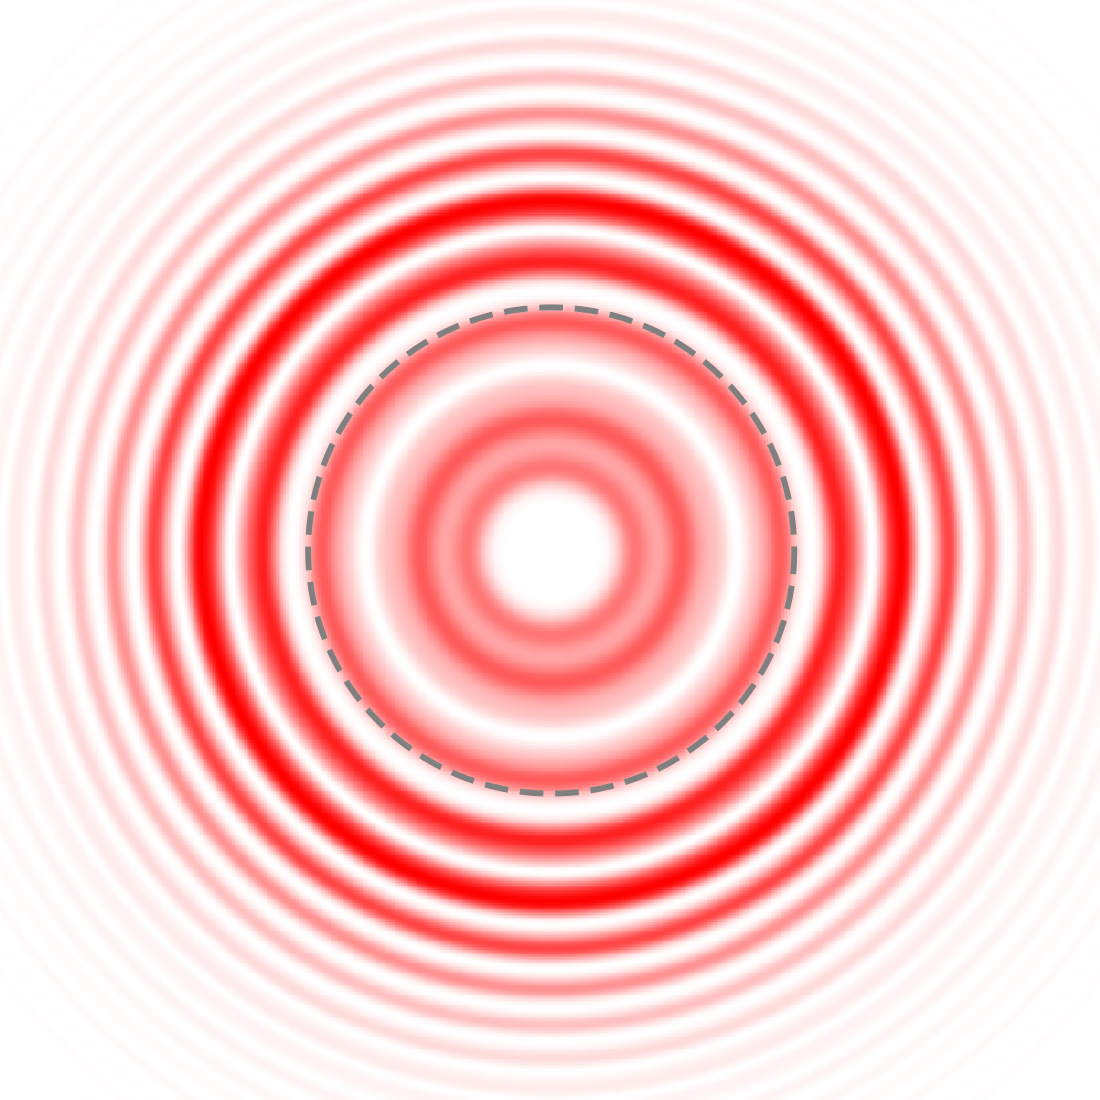
\includegraphics[width=40truemm]{slike/05_Fresnel_circ_k11_r1.png}\qquad
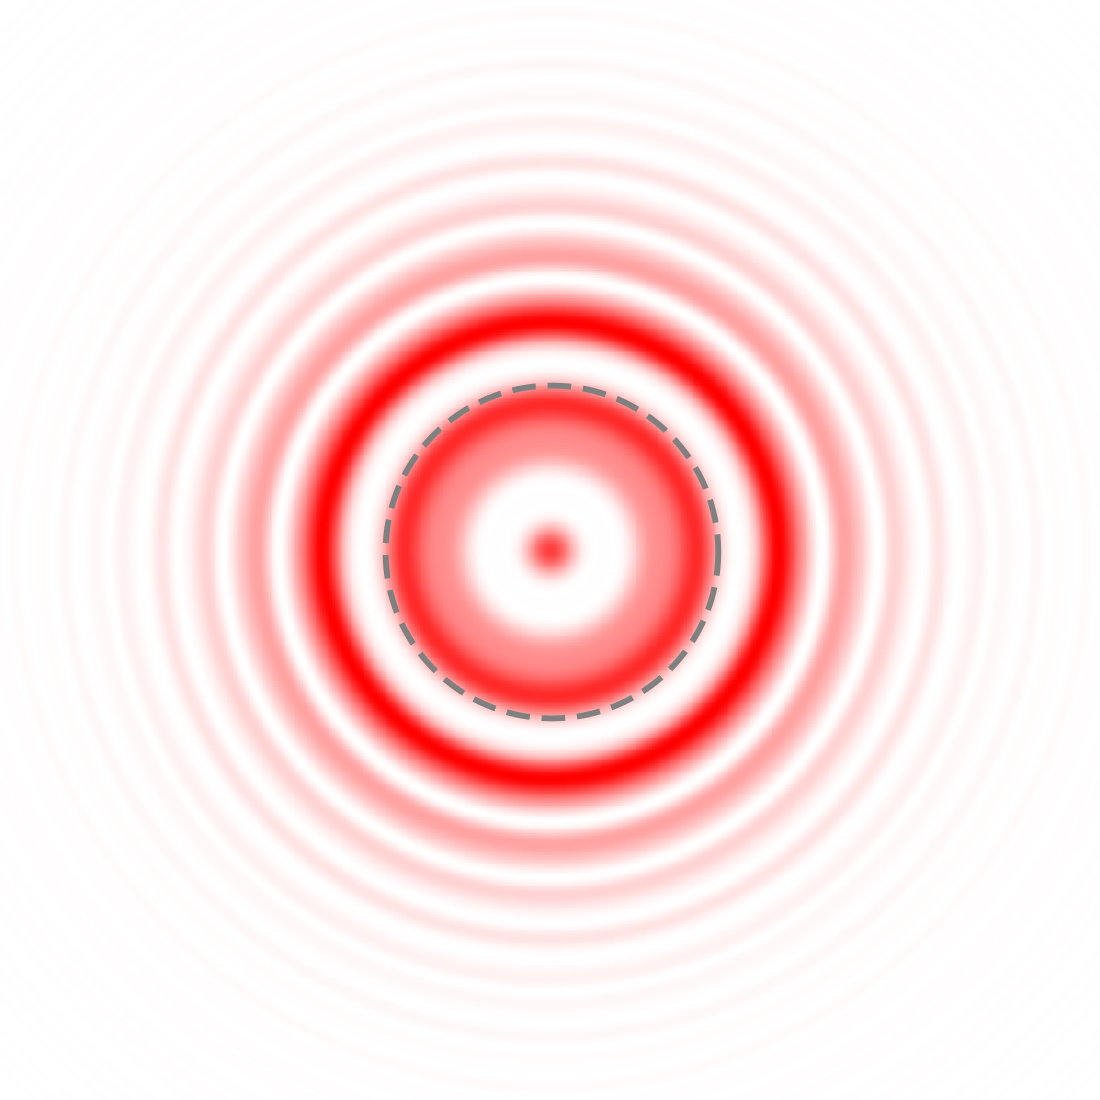
\includegraphics[width=40truemm]{slike/05_Fresnel_circ_k11_r07.png}\qquad
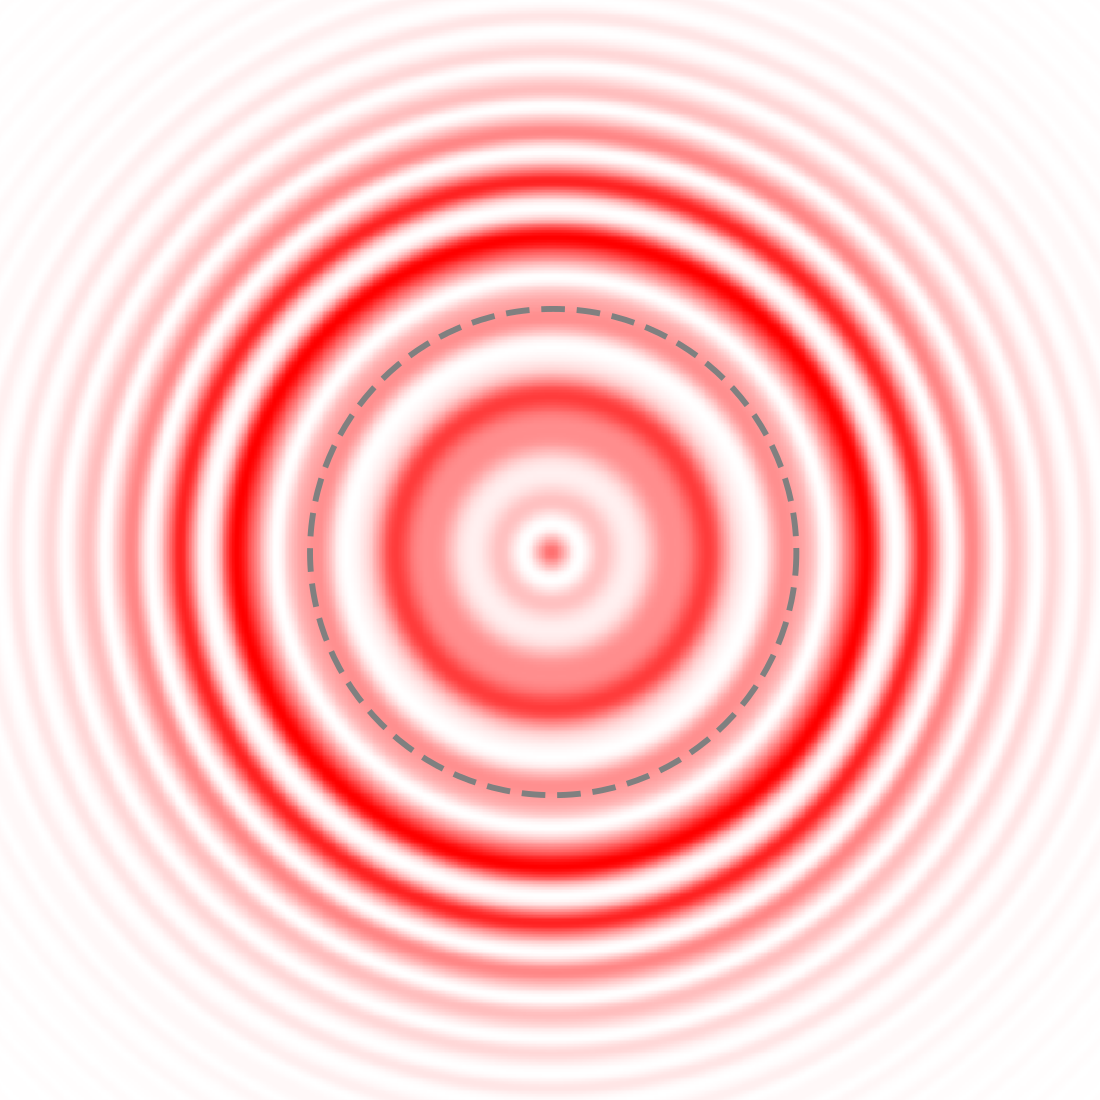
\includegraphics[width=40truemm]{slike/05_Fresnel_circ_k10_r1.png}\qquad
\caption{Simulacija uklonske slike na okrogli odprtini v Fresnelovem približku (levo).
Če spremenimo polmer odprtine (sredina) ali oddaljenost opazovalne ravnine (desno),
se uklonska slika spremeni. Črtkana črta označuje velikost odprtine.}
\label{fig:05_cirkularna_sim}
\end{figure}

\subsection*{Fresnelova uklonska leča}
Spoznali smo, da se prispevki sekundarnih valov iz posameznih Fresnelovih con izmenično
seštevajo in odštevajo. Če ohranimo v ravnini $xy$ le tiste kolobarje, ki so ali samo 
lihi ali samo sodi, se prispevki iz vseh obstoječih con le seštevajo (slika~\ref{fig:05_FresCona3}) in
gostota svetlobnega toka v točki $P_0$ je dosti večja, kot bi bila 
v primeru, če bi izvor svetlobe točko osvetljeval neposredno. Conska plošča torej 
deluje kot zbiralna leča. Izračunajmo njeno goriščno razdaljo. 
\begin{figure}[ht]
\centering

\includegraphics[width=40truemm]{slike/05_FresLeca.png}
\caption{Shema Fresnelove uklonske leče, ki je sestavljena iz lihih Fresnelovih con. }
\label{fig:05_lecaFr}
\end{figure}

Goriščno razdaljo uklonske leče izračunamo iz pogoja, da nastane slika 
žarkov, ki na lečo vpadajo iz neskončnosti ($z_0'\to \infty$), pri $z_0 = f$. Izhajamo 
iz enačbe~(\ref{eq:05_80}) in dobimo:
\beq
\frac{1}{L} = \frac{1}{z_0'}+ \frac{1}{z_0}= \frac{1}{z_0} = \frac{1}{f}\qquad \mathrm{oziroma}\qquad L=f.
\label{eq:05_91}
\eeq
Z uporabo enačbe~(\ref{eq:05_84a}) izračunamo goriščno razdaljo leče:
\beq
f = \frac{a_1^2}{\lambda}.
\label{eq:05_92}
\eeq
Kadar je Fresnelova conska plošča sestavljena iz zelo velikega števila Fresnelovih con, za izračun goriščne
razdalje zadošča, da poznamo polmer največjega kolobarja in približno razliko med polmeri zunanjih kolobarjev. Poglejmo, zakaj.

Upoštevamo izraz za polmer $N$-tega kolobarja (enačba~\ref{eq:05_90}) in zapišemo:  
\beq
a_{N+1}^2 - a_N^2 = \lambda (N+1)L - \lambda NL = \lambda L = a_1^2. 
\label{eq:05_93}
\eeq
Po drugi strani velja:
\beq
a_{N+1}^2 - a_N^2 = \left(a_{N+1}+a_N\right)\left(a_{N+1}- a_N\right) \approx 2a_N\Delta a_N.
\label{eq:05_94}
\eeq
Od tod sledi:
\beq
f = \frac{a_1^2}{\lambda} = \frac{2 a_N\Delta a_N}{\lambda}.
\label{eq:05_95}
\eeq
V izrazu za goriščno razdaljo Fresnelovih uklonskih leč neposredno nastopa valovna dolžina svetlobe, 
zato so za belo svetlobo zaradi velike kromatične aberacije praktično neuporabne. Uporablja se jih
predvsem za zbiranje svetlobe, kadar nimamo možnosti izdelave navadnih leč, na primer za rentgenske
žarke.
\end{example}

\begin{example}{\bf Fresnelov uklon na pravokotni reži.}
Kot drugi primer uporabe Fresnelovega uklonskega približka izračunajmo uklonsko sliko 
na pravokotni reži. Oz $z$ izberemo tako, da točkasti izvor svetlobe $S$ in
opazovalna točka $P_0$  ležita na njej, pravokotna reža s
koordinatami $x_1<x<x_2$ in $y_1<y<y_2$ pa naj leži v objektni
ravniki, ki je pravokotna na zveznico med točkama $S$ in $P_0$ (slika~\ref{fig:05_FresPravokot}).
\begin{figure}[ht]
\centering
\def\svgwidth{100truemm} 
\input{slike/05_Fres_kv_koor.pdf_tex}
\caption{K računu Fresnelovega uklona, ko izvor in detektor ležita na optični osi, v objektni ravnini
pa je kvadratna odprtina.}
\label{fig:05_FresPravokot}
\end{figure}

Fresnelov uklonski integral (enačba~\ref{eq:Fresnel}) za primer, ko izvor in detektor ležita
na optični osi, zapišemo kot:
\beq
E(0,0, z_0) = \frac{1}{i\lambda} \frac{\tilde{E}_0 e^{ikz_0'+ikz_0}}{z_0'z_0} 
\int_{x_1}^{x_2}\!\!\!\int_{y_1}^{y_2} e^{\frac{ik(x^2+y^2)}{2L}}  dx\,dy,
\label{eq:05_96}
\eeq
pri čemer je $L$ določen z enačbo~(\ref{eq:05_80}).

Osredotočimo se na dvojni integral, 
ki ga zapišemo v obliki:
\beq
E(P_0) \propto \int_{u_1}^{u_2} e^{i\frac{\pi}{2}u^2} du
\int_{v_1}^{v_2} e^{i\frac{\pi}{2}v^2} dv,
\label{eq:05_97}
\eeq
pri čemer sta spremenljivki, ki smo jih uvedli, enaki:
\beq
u = \sqrt{\frac{k}{\pi L}}\,x \qquad \mathrm{in} \qquad v = \sqrt{\frac{k}{\pi L}}\,y.
\label{eq:05_98}
\eeq
Zapisana integrala (enačba~\ref{eq:05_97}) izrazimo s Fresnelovima integraloma $C(u)$ in $S(u)$.

\begin{remark}
Fresnelova integrala sta oblike:
\beq
C(u) = \int_0^u \cos\left(\frac{1}{2}\pi x^2\right) dx \qquad \mathrm{in} \qquad 
S(u) = \int_0^u \sin\left(\frac{1}{2}\pi x^2\right) dx. 
\label{eq:05_99}
\eeq
\begin{figure}[ht]
\centering
\def\svgwidth{140truemm} 
\input{slike/05_FresC.pdf_tex}
\caption{Fresnelova integrala $C(u)$ in $S(u)$}
\label{fig:05_CS}
\end{figure}
Funkciji $C(u)$ in $S(u)$ sta transcendentni funkciji, ki ju moramo izračunati 
numerično (slika~\ref{fig:05_CS}). Obe funkciji sta lihi in $C(0)=S(0)=0$. 
V limitnih primerih velja $C(\infty) = 1/2$ in $C(-\infty) = -1/2$ ter enako za $S$. 
Integral, ki ga moramo izračunati, izrazimo s Fresnelovima integraloma: 
\beq
\int_{0}^{u} e^{i\frac{\pi}{2}u^2} du = C(u)+iS(u).
\label{eq:05_100}
\eeq
\end{remark}
\vglue4truemm
Jakost električnega polja uklonjene svetlobe (enačba~\ref{eq:05_97}) 
na pravokotni odprtini s Fresnelovima integraloma zapišemo kot:
\beq
\left. E(P_0) \propto \left( C(u) + iS(u) \right) \right|_{u_1}^{u_2} \cdot 
\left. \left( C(v) + iS(v) \right) \right|_{v_1}^{v_2},
\label{eq:05_101}
\eeq
intenziteto uklonske slike pa kot:
\beq
j(P_0)  = \frac{j_0}{4} \left(\!\!\left(C(u_2) -C(u_1)\!\right)^2 + \left(S(u_2) -
S(u_1)\!\right)^2\right)\!\!
\left(\!\!\left(C(v_2) -C(v_1)\!\right)^2 + \left(S(v_2) -S(v_1)\!\right)^2\right)\!\!.
\label{eq:05_101a}
\eeq
Primer Fresnelove uklonske slike na kvadratni odprtini, ki je postavljena simetrično
glede na optično os, je prikazan na sliki~\ref{fig:05_FrKv}.
\begin{figure}[ht]
\centering
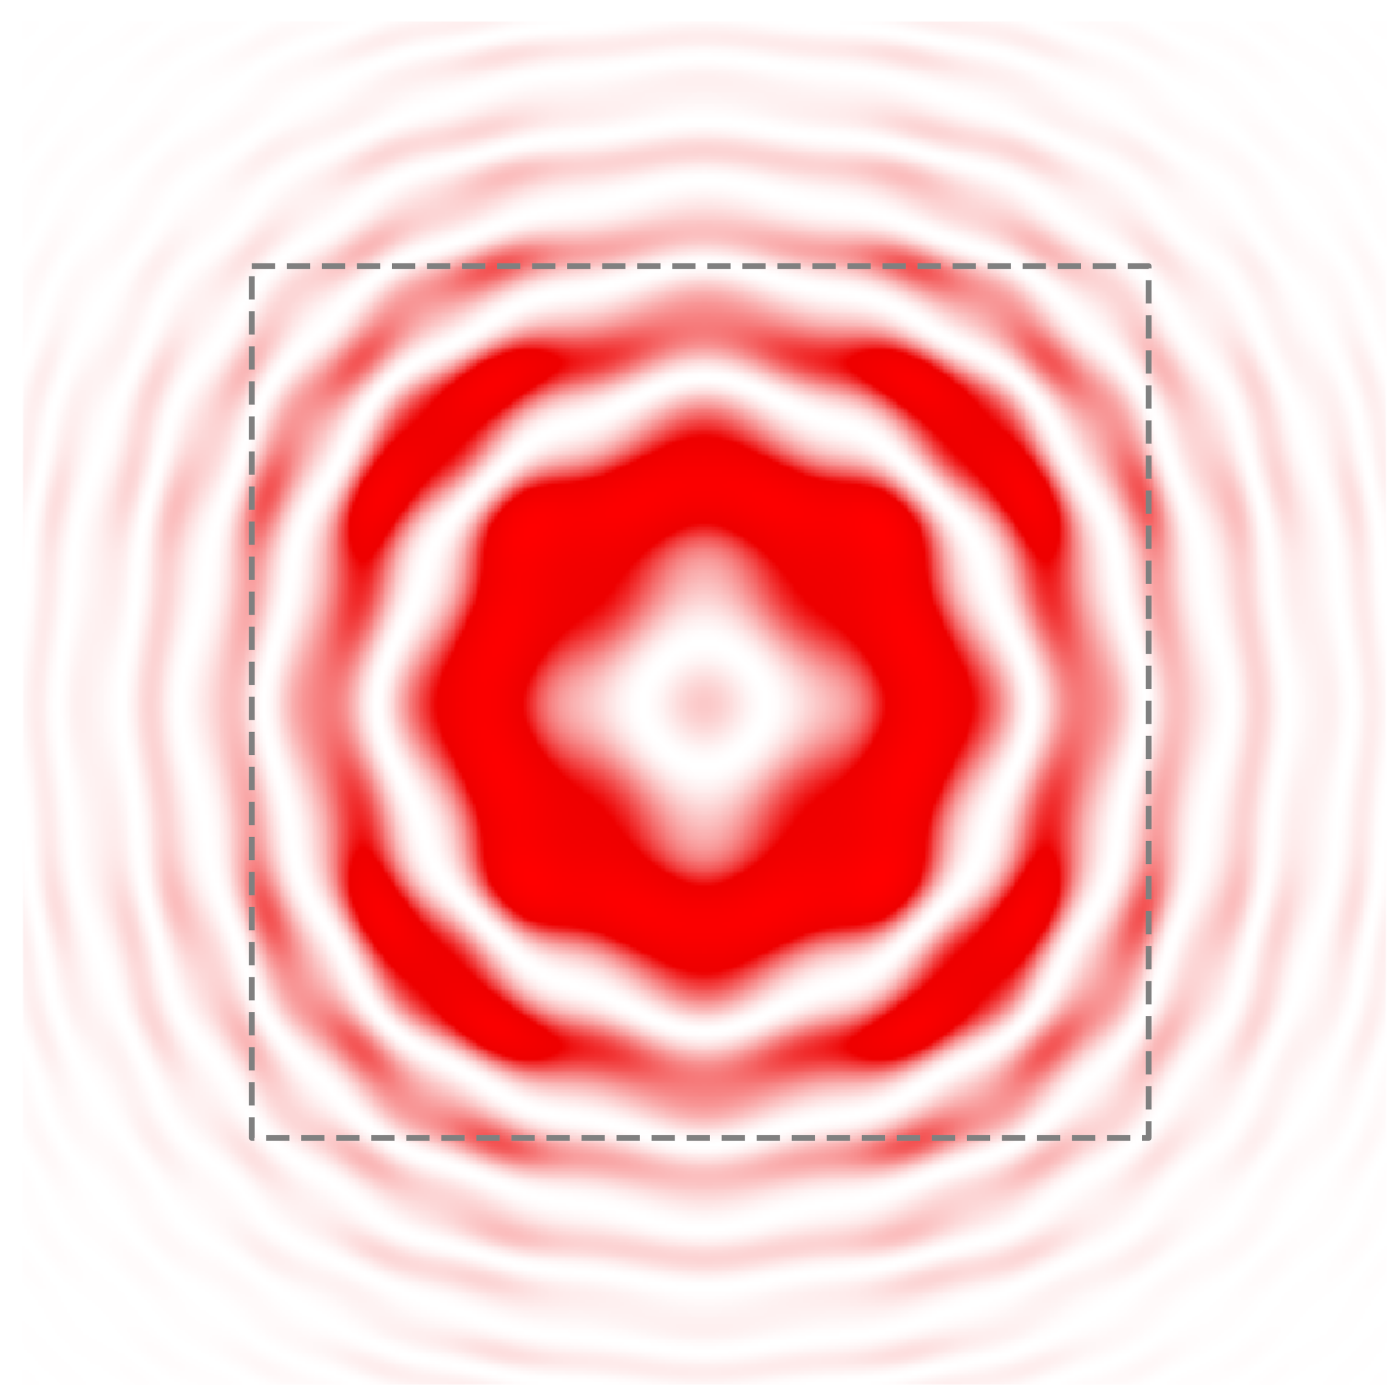
\includegraphics[width=50truemm]{slike/05_FresKvadrat.png}
\caption{Fresnelova uklonska slika na kvadratni odprtini na danem mestu. 
Črtkana črta označuje velikost odprtine.}
\label{fig:05_FrKv}
\end{figure}
Kot je značilno za Fresnelov uklon, se uklonska slika na kvadratni odprtini spreminja
z oddaljenostjo od odprtine. 

Na povsem enak način kot smo izračunali Fresnelovo uklonsko sliko na pravokotni odprtini,
izračunamo uklonsko sliko na reži. Pri računu se omejimo
na le eno dimenzijo in en integral. Na sliki~\ref{fig:05_FrReza} je prikazanih nekaj 
primerov Fresnelovih uklonskih slik za reže različnih širin. 
\begin{figure}[!h]
\centering
\def\svgwidth{140truemm} 
\input{slike/05_Fresnek_Reza.pdf_tex}
\caption{Fresnelova uklonska slika na reži za različne širine rež. Uklonska slika
zelo ozke reže je podobna Fraunhoferjevi uklonski sliki, pri večjih se od Fraunhoferjeve 
znatno razlikuje. Črtkana črta označuje velikost odprtine. Desno so simulacije uklonskih
slik na režah.}
\label{fig:05_FrReza}
\end{figure}
\vglue5truemm

\end{example}

\begin{example}{\bf Fresnelov uklon na ostrem robu.}
Izračunajmo še Fresnelovo uklonsko sliko, ki nastane na ostrem ravnem robu. Primer
lahko obravnavamo kot uklon na reži, pri čemer eno mejo integracije postavimo v neskončnost:
$x_1 \to -\infty$ oziroma $u_1 \to -\infty$. Druga meja naj bo $x_2 = d$ oziroma 
$u_2  = d\sqrt{k/\pi L}$. Fresnelova uklonska slika v točki na optični osi 
je v splošnem (enačba~\ref{eq:05_101}):
\beq
\left. E(P_0) \propto \left( C(u) + iS(u) \right) \right|_{-\infty}^{u_2} = 
C(u_2) + i S(u_2) + 1/2 + i/2,
\label{eq:05_102}
\eeq
od koder sledi:
\beq
j(P_0)  = \frac{j_0}{2}\left(\!\!\left(C(u_2) + \frac{1}{2}\right)^2 + \left(S(u_2) + \frac{1}{2}\right)^2\right)\!\!.
\label{eq:05_103}
\eeq
Zapisana gostota svetlobnega toka opisuje vrednost na danem mestu na optični osi. 
Celotno uklonsko sliko na robu dobimo tako, da namesto premikanja opazovalne točke $P_0$ vzdolž osi 
$\xi$, točko $P_0$ ohranjamo na optični osi in premikamo rob zaslona 
v smeri osi $x$. Pri tem negativne vrednosti $d$ ustrezajo geometrijski senci. 
\begin{figure}[ht]
\centering
\def\svgwidth{140truemm} 
\input{slike/05_Fresnel_rob.pdf_tex}
\caption{Fresnelova uklonska slika na ostrem robu. Intenziteta v odvisnosti od lege (levo),
simulacija (desno zgoraj) in fotografija (desno spodaj).}
\label{fig:05_FresRob}
\vglue-4truemm
\end{figure}

Fresnelova uklonska slika je prikazana na sliki~\ref{fig:05_FresRob}, pri čemer navpična
črtkana črta označuje lego roba. Slika v odprtini je oscilirajoča in se v veliki oddaljenosti
od roba približuje vrednosti $j_0$. V senci intenziteta hitro pojema, na robu je vrednost
$0,25 j_0$.  
\vglue-2truemm
\begin{remark}
Danes uklonske slike računamo numerično, nekoč pa so uporabljali tabele ali 
grafično upodobitev. Nazorna grafična predstavitev Fresnelovih 
integralov $C(u)$ in $S(u)$, ki jih uporabimo za izračun uklonske slike 
na pravokotnih odprtinah, režah ali na robu, je v obliki Eulerjeve ali Cornujeve spirale. 
Fresnelova integrala prikažemo grafično tako, da narišemo
krivuljo v parametrični obliki $C(t), S(t)$ v 2D-ravnini. 
\begin{figure}[ht]
\centering
\def\svgwidth{80truemm} 
\input{slike/05_Fresnel_Cornu.pdf_tex}
\caption{Cornujeva spirala za izračun Fresnelovega uklonskega približka}
\label{fig:05_Cornu}
\vglue-2truemm
\end{figure}

Poglejmo za primer Fresnelov uklon na ostrem robu. Primer je enodimenzionalen in 
intenziteta uklonjene svetlobe je sorazmerna vsoti 
kvadratov razlik integralov v končni in začetni točki (enačba~\ref{eq:05_103}). Matematično
gledano je to ravno dolžina daljice, ki na krivulji povezuje začetno in končno točko.
Začetna točka je pri $u \to -\infty$, kar ustreza točki $(-1/2, -1/2)$ na spirali. 
Končna točka je pri $u_2$, ki za izračun celotne uklonske slike potuje po spirali
od enega do drugega konca. Na začetku dolžina daljice (in z njo intenziteta uklonjene
svetlobe) počasi narašča (rumena črta), nato hitro naraste (zelena črta) do 
največje vrednosti, potem pa s premikanjem po spirali izmenično pojema in narašča
z vedno manjšo amplitudo (modra črta). Uklonska slika, ki jo dobimo, je enaka 
kot na sliki~\ref{fig:05_FresRob}. 
\end{remark}
\vglue-5truemm

\end{example}

\section{*Izpeljava Kirchhoffovega uklonskega integrala}
\label{chap:Kirchhoff}
Poglejmo za konec še matematično izpeljavo uklonskega integrala (enačba~\ref{eq:05_01}). 
Za izpeljavo bomo uporabili Greenov teorem, ki izhaja iz Gaussovega stavka. 

Naj bo $\mathbf{W}(\mathbf{r})$ poljubno zvezno in zvezno odvedljivo vektorsko
polje. Gaussov stavek pravi, da je integral po sklenjeni ploskvi enak
integralu divergence vektorskega polja po prostoru:
\beq
\oint_S \mathbf{W} \cdot d\mathbf{S} = \int_V \div\mathbf{W}\,dV.
\label{eq:05_48}
\eeq
Zapišimo  vektorsko polje $\mathbf{W}$ s skalarnima poljema $\Psi$ in $\Phi$
v obliki:
\beq
\mathbf{W}(\mathbf{r}) = \Psi \nabla \Phi - \Phi \nabla \Psi,
\label{eq:05_49}
\eeq
pri čemer sta funkciji $\Psi$ in $\Phi$ zvezni in dvakrat zvezno odvedljivi.
Potem velja:
\beq
\div \mathbf{W}= \Psi \nabla^2 \Phi - \Phi \nabla^2 \Psi. 
\label{eq:05_50}
\eeq
Enačbi~(\ref{eq:05_49}) in (\ref{eq:05_50}) vstavimo v Gaussov stavek 
(enačba~\ref{eq:05_48}) in dobimo Greenov teorem:
\beq
\oint_S \left(\Psi \nabla \Phi - \Phi \nabla \Psi\right) \cdot d\mathbf{S}  =
\int_V \left( \Psi \nabla^2 \Phi - \Phi \nabla^2 \Psi \right) dV.
\label{eq:05_51}
\eeq

Izberimo za $\Psi$ in $\Phi$ funkciji, ki predstavljata skalarni rešitvi
krajevnega dela valovne enačbe. Za ti dve funkciji torej veljata zvezi:
\beq
\nabla^2 \Psi + k^2 \Psi = 0 \qquad \mathrm{in} \qquad \nabla^2 \Phi + k^2 \Phi = 0.
\label{eq:05_52}
\eeq
Z upoštevanjem teh dveh zvez postane desni del Greenovega teorema 
(enačba~\ref{eq:05_51}) identično enak nič. Od tod sledi, da za funkciji $\Psi$ in $\Phi$,
ki sta rešitvi valovne enačbe, velja zveza:
\beq
\oint_S \left( \Psi\frac{\partial \Phi}{\partial \mathbf{n}} -
\Phi\frac{\partial \Psi}{\partial \mathbf{n}} \right) dS = 0.
\label{eq:05_53}
\eeq
Skalarni produkt med gradientom in normalo na ploskev $\mathbf{n}$ smo
zapisali kot smerni odvod:
\beq
\nabla\Phi \cdot d\mathbf{S} = \nabla \Phi \cdot \mathbf{n}\,dS = 
\frac{\partial \Phi}{\partial \mathbf{n}}\,dS.
\label{eq:05_53a}
\eeq

V skladu z Huygensovim  načelom si zamislimo, da funkcija $\Psi$ opisuje sferične valove, ki
izhajajo iz izhodišča $P_0$. Izkaže se, da je končni rezultat neodvisen od izbire
funkcije $\Psi$, je pa nedvomno najnazornejši, če za funkcijo $\Psi$ 
izberemo sferične valove v obliki:
\beq
\Psi = A \frac{e^{ikr}}{r},
\label{eq:05_54}
\eeq
pri čemer $A$ pomeni njeno amplitudo, $k$ je valovni vektor, $r$ pa je 
razdalja od izhodišča. Ker zapisana funkcija $\Psi$ 
v izhodišču pri $r=0$ divergira, moramo izhodišče
izvzeti iz računa, saj smo v začetku privzeli, da je funkcija $\Psi$
zvezno odvedljiva. Namesto po celotnem telesu torej integriramo 
po celotnem telesu, zmanjšanem za kroglo s 
polmerom $\varepsilon$ okoli točke $P_0$ (slika~\ref{fig:05_Green}).
\begin{figure}[ht]
\centering
\def\svgwidth{70truemm} 
\input{slike/05_Green1.pdf_tex}
\caption{K izračunu Greenovega teorema, pri katerem moramo zaradi divergence krogelnega
vala $\Psi$ v izhodišču od integracije odvzeti majhno kroglico s polmerom $\varepsilon$.}
\label{fig:05_Green}
\end{figure}

Celotna integracijska ploskev je tako sestavljena iz zunanje ploskve
$S$ in notranje krogle $S_\varepsilon$. Enačbo~(\ref{eq:05_53}) z uporabo
enačbe~(\ref{eq:05_54}) prepišemo v:
\beq
\oint_S \left( \frac{e^{ikr}}{r}\frac{\partial \Phi}{\partial \mathbf{n}} -
\Phi\frac{\partial}{\partial \mathbf{n}}\left( \frac{e^{ikr}}{r} \right)\!\! \right) dS -
\oint_{S\varepsilon} \left( \frac{e^{ikr}}{r}\frac{\partial \Phi}{\partial \mathbf{n}} -
\Phi\frac{\partial}{\partial \mathbf{n}}\left( \frac{e^{ikr}}{r} \right)\!\! \right)r^2 d\Omega = 0.
\label{eq:05_55}
\eeq
Ker je notranja ploskev krogla, je smer normale na ploskev $\mathbf{n}$ enaka smeri $\mathbf{r}$ in
odvod preprosto izračunamo:
\beq
\frac{\partial}{\partial r}\left( \frac{e^{ikr}}{r}\right)  = ik \frac{e^{ikr}}{r} - \frac{e^{ikr}}{r^2}.
\label{eq:05_56}
\eeq
Drugi integral v enačbi~(\ref{eq:05_55}) potem prepišemo v:
\beq
\oint_{S\varepsilon} \left( \frac{e^{ikr}}{r}\frac{\partial \Phi}{\partial \mathbf{n}}r^2 -
ik\frac{e^{ikr}}{r}r^2\,\Phi + \frac{e^{ikr}}{r^2}r^2\,\Phi\right) d\Omega.
\label{eq:05_57}
\eeq
V limiti, ko gre polmer notranje krogle $\varepsilon \to 0$, gresta tako prvi kot 
drugi člen proti 0, tretji člen pa gre proti vrednosti $4\pi\, \Phi(P_0)$. Faktor $4\pi$ 
dobimo pri integraciji po polnem kotu, eksponent pa je za majhne polmere enak $1$.

Rezultat iz enačbe~(\ref{eq:05_57}) vstavimo v enačbo~(\ref{eq:05_55}) in dobimo:
\beq
\Phi(P_0) = \frac{1}{4\pi} \oint_S \left( \frac{e^{ikr}}{r}\frac{\partial \Phi}{\partial \mathbf{n}} -
\Phi\frac{\partial}{\partial \mathbf{n}}\left( \frac{e^{ikr}}{r} \right)\!\! \right) dS.
\label{eq:05_58}
\eeq
S to enačbo smo skalarno polje $\Phi$ v točki $P_0$ 
izrazili s skalarnim poljem $\Phi$ na sklenjeni površini $S$, ki to točko obdaja. Če torej 
poznamo polje na neki poljubni sklenjeni ploskvi okoli dane točke, lahko polje v tej 
točki izračunamo.

Obravnavajmo točkasti izvor valovanja, ki iz točke $P$ oddaja krogelne valove 
oblike:
\beq
\Phi = \tilde{E}_0\frac{e^{ikr'}}{r'}.
\label{eq:05_58a}
\eeq
Krogelni valovi vpadajo na objektni zaslon z odprtino, 
naša naloga pa je izračunati uklonjeno polje v točki $P_0$ na drugi strani zaslona 
(slika~\ref{fig:05_Kirchhoff}). 
Spomnimo se, da za izračun polja v točki $P_0$ zadošča, če poznamo polje na neki
sklenjeni ploskvi $S$, ki to točko obdaja.

\begin{figure}[ht]
\centering
\def\svgwidth{80truemm} 
\input{slike/05_Green2.pdf_tex}
\caption{K izpeljavi Kirchhofovega integrala. Privzamemo, da je prispevek k integralu po 
ploskvi $S$, po kateri integriramo, povsod enak nič, razen v odprtini $S_A$. Za izračun
polja v točki $P_0$ tako zadošča poznati polje v odprtini.}
\label{fig:05_Kirchhoff}
\end{figure}

Integracijsko ploskev okoli točke $P_0$ izberemo tako, da delno poteka po zaslonu
in delno zelo daleč od zaslona. Privzamemo, da je drugi del integracijske ploskve tako oddaljen
od zaslona in opazovalne točke, da so prispevki polja $\Phi$ na njem zanemarljivo majhni. 
Ostane torej le integracija po objektni ravnini. Tudi tukaj naredimo nekaj približkov.
Privzamemo, da sta polje in njegov odvod na zaslonu povsod, razen v odprtini, enaka nič. 
Drugi približek pravi, da je polje v odprtini tako, kot da zaslona ne bi bilo. 

Za izračun polja v točki $P_0$ tako zadošča izračunati integral le po površini odprtine $S_A$. 
Izračunajmo najprej smerni odvod, ki ga potrebujemo za izračun integrala (enačba~\ref{eq:05_58}):
\beq
\frac{\partial \Phi}{\partial \mathbf{n}} = (\nabla \Phi)\cdot \mathbf{n} = 
\frac{\partial \Phi}{\partial r'} \frac{\mathbf{r'}}{r'}\cdot \mathbf{n} = \frac{\partial \Phi}{\partial r'} 
\cos\left(\mathbf{r'},\mathbf{n}\right)\!.
\label{eq:05_59}
\eeq
Z $\left(\mathbf{r'},\mathbf{n}\right)$ smo označili kot med vektorjema $\mathbf{r}'$ in normalo
na ploskev $\mathbf{n}$. Po dogovoru normala na ploskev vedno kaže ven iz ploskve, zato
na odprtini kaže proti strani izvora. 

Izračunajmo odvod funkcije $\Phi$ (enačba~\ref{eq:05_58a}):
\beq
\frac{\partial \Phi}{\partial r'} = \frac{\partial}{\partial r'}\left(\tilde{E}_0\frac{e^{ikr'}}{r'}\right) = 
\tilde{E}_0\frac{ikr'-1}{r'^2}e^{ikr'} \approx \tilde{E}_0\frac{ik}{r'}e^{ikr'}.
\label{eq:05_60}
\eeq
Privzeli smo, da je razdalja $r'$ bistveno večja od valovne dolžine svetlobe, in 1 v števcu zanemarilli. 
Podobno izračunamo tudi drugi člen v enačbi~(\ref{eq:05_58}) in upoštevamo, da je $\lambda \ll r$. Dobimo:
\beq
\frac{\partial}{\partial \mathbf{n}}\left( \frac{e^{ikr}}{r} \right) = 
\cos\left(\mathbf{r},\mathbf{n}\right) \frac{\partial}{\partial r} \left( \frac{e^{ikr}}{r} \right) \approx
\cos\left(\mathbf{r},\mathbf{n}\right) \frac{ik}{r}e^{ikr}.
\label{eq:05_60a}
\eeq
Uporabimo enačbe~(\ref{eq:05_59}, \ref{eq:05_60} in \ref{eq:05_60a}) in jih vstavimo v enačbo~(\ref{eq:05_58}). Dobimo:
\beq
\Phi(P_0) = \frac{1}{4\pi} \int_{S_A} \left( \frac{e^{ikr}}{r}\,\tilde{E}_0\, \frac{ik}{r'}e^{ikr'} \cos\left(\mathbf{r'},\mathbf{n}\right)-\tilde{E}_0
\frac{e^{ikr'}}{r'} \frac{ik}{r}e^{ikr} \cos\left(\mathbf{r},\mathbf{n}\right)  \right) dS,
\label{eq:05_61}
\eeq
od koder sledi:
\boxeq{eq:05_62}{
\Phi(P_0) = \frac{ik}{4\pi} \int_{S_A} \tilde{E}_0\,\frac{e^{ikr}e^{ikr'}}{rr'}
\left( \cos\left(\mathbf{r'},\mathbf{n}\right) - \cos\left(\mathbf{r},\mathbf{n}\right) \right) dS.
}
Razliko kosinusov imenujemo tudi oblikovni faktor. V geometriji, ki smo jo privzeli, navadno velja
\beq
\cos\left(\mathbf{r'},\mathbf{n}\right) \approx -1 \qquad \mathrm{in} \qquad \cos\left(\mathbf{r},\mathbf{n}\right) \approx 1.
\label{eq:05_63}
\eeq
Potem se integral iz enačbe~(\ref{eq:05_62}) poenostavi v:
\beq
\Phi(P_0) = - \frac{2ik}{4\pi} \int_{S_A} \tilde{E}_0 \frac{e^{ikr}e^{ikr'}}{rr'} dS = 
\frac{1}{i\lambda} \int_{S_A}\tilde{E}_0 \frac{e^{ikr}e^{ikr'}}{rr'} dS.
\label{eq:05_64}
\eeq
S tem smo izpeljali predfaktor v prvotni enačbi~(\ref{eq:05_01}).

\begin{figure}[ht]
\centering
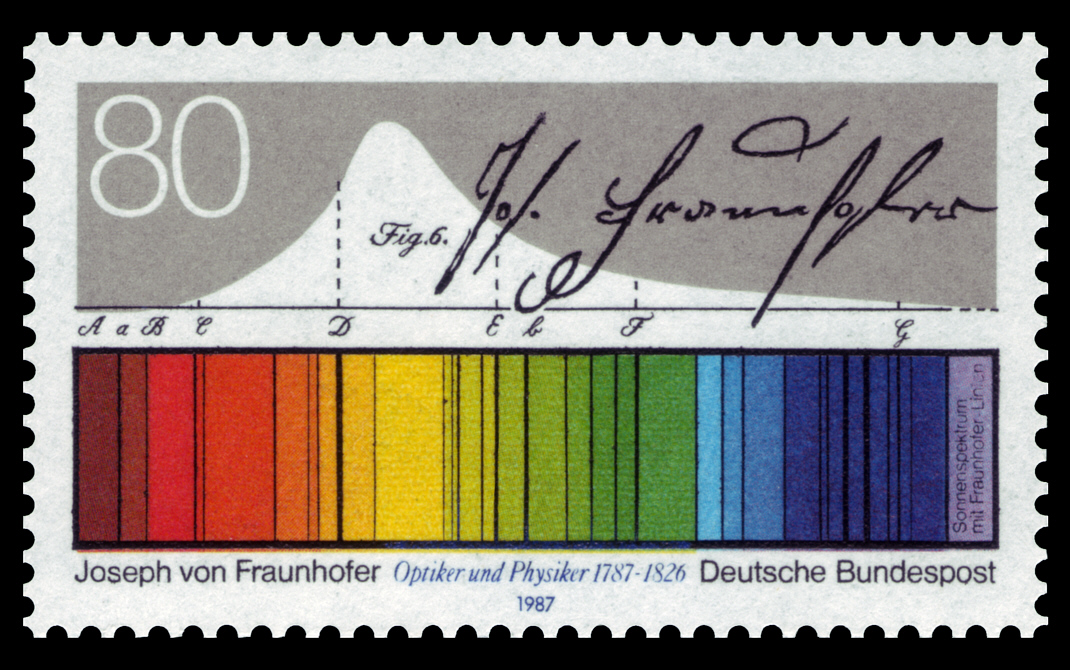
\includegraphics[width=90truemm]{slike/05_Znamka.jpg}
\caption{Znamka, ki je izšla ob 200-letnici rojstva Josepha von Fraunhoferja. Njegova natančna
izdelava optičnih elementov in uklonskih mrežic je omogočila opazovanje spektra bele svetlobe 
s Sonca in analizo manjkajočih črt. Vir: Deutsche Bundespost, Wikimedia.}
\label{fig:05_znamka}
\end{figure}
